\documentclass[a4paper, 10pt]{book}
\usepackage[a4paper, total={6in, 8in}]{geometry}

\usepackage{amssymb}
\usepackage[figuresright]{rotating}

%\usepackage{fontspec}
\usepackage{lmodern}
\usepackage{lipsum}
\usepackage{psl-cover}

% my packages:
\usepackage[utf8]{inputenc}
\usepackage[english]{babel}
\usepackage{amsmath}
\usepackage{amsfonts}
\usepackage{amssymb}
\usepackage{graphicx}
\usepackage{siunitx}
\sisetup{math-micro=\text{µ},text-micro=µ}
\usepackage[euler]{textgreek}
\usepackage{subcaption}
\usepackage{booktabs}
\usepackage{soul}
\usepackage{enumitem}
\usepackage{bm}

\usepackage{notations}

\usepackage{import}
\usepackage{example}
\usepackage{graphicx}
\usepackage{amsmath}
\usepackage{float}
\usepackage{amssymb}
\usepackage{xcolor}
\usepackage{hyperref}
\usepackage{longtable}
\usepackage{listings}
\usepackage{multicol}
\usepackage{import}
\usepackage{comment}
\usepackage{ulem}
\usepackage{booktabs,xltabular}
\usepackage{longtable} 

\title{Insérer ici l'intitulé du sujet de thèse}

\author{Martinus Putra Widjaja}

\institute{MINES ParisTech}
\doctoralschool{Ingénierie des Systèmes, Matériaux, Mécanique, Energétique}{621}
\specialty{Voir spécialités ED}
\date{jj mois aaaa}

%% cotutelle
% \entitle{Thesis Subject in English}
% \otherinstitute{CEA Saclay}
% \logootherinstitute{logo-institute}

\jurymember{1}{Prénom NOM}{Titre, établissement}{Président}
\jurymember{2}{Prénom NOM}{Titre, établissement}{Rapporteur}
\jurymember{3}{Prénom NOM}{Titre, établissement}{Rapporteur}
\jurymember{4}{Prénom NOM}{Titre, établissement}{Examinateur}
\jurymember{5}{Prénom NOM}{Titre, établissement}{Examinateur}
\jurymember{6}{Prénom NOM}{Titre, établissement}{Examinateur}
\jurymember{7}{Prénom NOM}{Titre, établissement}{Examinateur}
\jurymember{8}{Alain THIONNET}{Titre, établissement}{Directeur de thèse}
% \jurymember{9}{Prénom NOM}{Titre, établissement}{Invité}
% \jurymember{10}{Prénom NOM}{Titre, établissement}{Invité}

\frabstract{
  Cuius acerbitati uxor grave accesserat incentivum,
  germanitate Augusti turgida supra modum, quam Hannibaliano
  regi fratris filio antehac Constantinus iunxerat pater,
  Megaera quaedam mortalis, inflammatrix saevientis adsidua,
  humani cruoris avida nihil mitius quam maritus; qui paulatim
  eruditiores facti processu temporis ad nocendum per
  clandestinos versutosque rumigerulos conpertis leviter
  addere quaedam male suetos falsa et placentia sibi
  discentes, adfectati regni vel artium nefandarum calumnias
  insontibus adfligebant.

  Saraceni tamen nec amici nobis umquam nec hostes optandi,
  ultro citroque discursantes quicquid inveniri poterat
  momento temporis parvi vastabant milvorum rapacium similes,
  qui si praedam dispexerint celsius, volatu rapiunt celeri,
  aut nisi impetraverint, non inmorantur.

  Vita est illis semper in fuga uxoresque mercenariae
  conductae ad tempus ex pacto atque, ut sit species
  matrimonii, dotis nomine futura coniunx hastam et
  tabernaculum offert marito, post statum diem si id elegerit
  discessura, et incredibile est quo ardore apud eos in
  venerem uterque solvitur sexus.

  Sed tamen haec cum ita tutius observentur, quidam vigore artuum
  inminuto rogati ad nuptias ubi aurum dextris manibus cavatis
  offertur, inpigre vel usque Spoletium pergunt.\ haec nobilium sunt
  instituta.
}

\enabstract{
  Verum ad istam omnem orationem brevis est defensio. Nam
  quoad aetas M. Caeli dare potuit isti suspicioni locum, fuit
  primum ipsius pudore, deinde etiam patris diligentia
  disciplinaque munita. Qui ut huic virilem togam deditšnihil
  dicam hoc loco de me; tantum sit, quantum vos existimatis;
  hoc dicam, hunc a patre continuo ad me esse deductum; nemo
  hunc M. Caelium in illo aetatis flore vidit nisi aut cum
  patre aut mecum aut in M. Crassi castissima domo, cum
  artibus honestissimis erudiretur.

  Et eodem impetu Domitianum praecipitem per scalas itidem
  funibus constrinxerunt, eosque coniunctos per ampla spatia
  civitatis acri raptavere discursu.\ iamque artuum et
  membrorum divulsa conpage superscandentes corpora mortuorum
  ad ultimam truncata deformitatem velut exsaturati mox
  abiecerunt in flumen.

  Erat autem diritatis eius hoc quoque indicium nec obscurum
  nec latens, quod ludicris cruentis delectabatur et in circo
  sex vel septem aliquotiens vetitis certaminibus pugilum
  vicissim se concidentium perfusorumque sanguine specie ut
  lucratus ingentia laetabatur.

  Ego vero sic intellego, Patres conscripti, nos hoc tempore in
  provinciis decernendis perpetuae pacis habere oportere rationem. Nam
  quis hoc non sentit omnia alia esse nobis vacua ab omni periculo
  atque etiam suspicione belli?
}

\frkeywords{ Caesar licentia post honoratis haec adhibens urbium
  honoratis nullum Caesar.}
\enkeywords{ Delatus delatus nominatus
  onere aut trahebatur quod tenus et bonorum.}

\begin{document}

\maketitle{}

\tableofcontents
\listoffigures

% CHAPTER 2
\chapter{Chapter 01}
\label{section_chapter_xxx}

% les notations doivent faire partie de l'introduction
\section*{Notations}
\label{sec_notations}
%
%
%
\begin{longtable}{c l}
    \caption{Notation}
    \label{table_notation}
    \\
    \hline
    \textbf{Notation} & \textbf{Meaning}
    \\
    \hline
    $r$ & scalar variable
    \\
    $\tensori{r}$ & vector variable
    \\
    $\tensorii{r}$ & second order tensor variable
    \\
    $\tensoriv{r}$ & fourth order tensor variable
    \\
    $\mathfrak{R}$ & vector representation of some tensorial field $r / \tensori{r} / \tensorii{r} / \tensoriv{r}$
    \\
    $\mathbb{R}$ & matrix representation of some tensorial field $r / \tensori{r} / \tensorii{r} / \tensoriv{r}$
    \\
    $\tensorii{I}$ & identity tensor
    \\
    $\lVert \tensori{r} \rVert$ & euclidean norm
    \\
    $\nabla$ & Lagrangian gradient operator
    \\
    $\nabla \cdot$ & Lagrangian divergence operator
    \\
    $\otimes$ & tensorial diadic product
    \\
    $\cdot$ & scalar product
    \\
    $\delta r / \delta \tensori{r} / \delta \tensorii{r}$ & variation of the tensorial field $r / \tensori{r} / \tensorii{r}$
    \\
    $\hat{r} / \tensori{\hat{r}} / \tensorii{\hat{r}}$ & admissible virtual field associated with the quantity $r / \tensori{r} / \tensorii{r}$
    \\
    $r \vert_{\partial D} / \tensori{r} \vert_{\partial D} / \tensorii{r} \vert_{\partial D}$ & trace of the tensorial field $r / \tensori{r} / \tensorii{r}$ on some boundary domain $\partial D$
    \\
    $\bodyEul$ & solid body in its current configuration
    \\
    $\tensori{x}$ & a point in the current solid body
    \\
    $\loadEul$ & imposed weight in the current solid body
    \\
    $\dBodyEul{}{}$ & solid body boundary
    \\
    $\neumannBoundaryEul$ & Neumann part of the solid body boundary
    \\
    $\neumannEul{}$ & imposed traction on the Neumann boundary of the solid body
    \\
    $\dirichletBoundaryEul{}$ & Dirichlet part of the solid body boundary
    \\
    $\dirichletEul$ & imposed displacement on the Dirichlet boundary of the solid body
    \\
    $\bodyLag$ & solid body in its reference configuration
    \\
    $\tensori{X}$ & a point in the reference solid body
    \\
    $\loadLag$ & imposed weight in the solid body
    \\
    $\dBodyLag{}$ & solid body boundary
    \\
    $\neumannBoundaryLag$ & Neumann part of the solid body boundary
    \\
    $\neumannLag{}$ & imposed traction on the Neumann boundary of the solid body
    \\
    $\dirichletBoundaryLag{}$ & Dirichlet part of the solid body boundary
    \\
    $\dirichletLag$ & imposed displacement on the Dirichlet boundary of the solid body
    \\
    $\tensori{\Phi}$ & transformation mapping of the solid body
    \\
    $\tensori{u}$ & solid body displacement field
    \\
    $\tensorii{G}$ & solid body displacement gradient
    \\
    $\tensorii{F}$ & transformation mapping gradient of the solid body
    \\
    $\tensorii{P}$ & first Piola-Kirchoff stress tensor in the solid body 
    \\
    $\mecPotential_{\bodyLag}$ & mechanical free energy potential in the solid body 
    \\
    $\cell$ & a cell, as a subdomain of the solid body
    \\
    $h_T$ & cell diameter
    \\
    $\dCell{}$ & cell boundary
    \\
    $\tensori{n}$ & normal vector to the cell boundary
    \\
    $F$ & a face of the cell, belonging to the cell boundary
    \\
    $\neumannCell{}$ & Neumann part of the cell boundary
    \\
    $\neumannCellLoad{}$ & imposed traction on the Neumann boundary of the cell
    \\
    $\dirichletCell{}$ & Dirichlet part of the cell boundary
    \\
    $\dirichletCellLoad$ & imposed displacement on the Dirichlet boundary of the cell
    \\
    $\tensori{u}{}_{\cell}$ & cell displacement field
    \\
    $\tensori{u}{}_{\dCell}$ & cell boundary displacement field
    \\
    $\tensori{u}{}_{F}$ & face boundary displacement field
    \\
    $\tensorii{G}{}_{\cell}$ & cell displacement gradient
    \\
    $\tensorii{F}{}_{\cell}$ & transformation mapping gradient of the cell
    \\
    $\tensorii{P}{}_{\cell}$ & first Piola-Kirchoff stress tensor in the cell
    \\
    $\tensori{u}{}_{\cell}^h$ & cell displacement field
    \\
    $\tensori{u}{}_{\dCell}^h$ & cell boundary displacement field
    \\
    $\tensori{u}{}_{F}^h$ & face boundary displacement field
    \\
    $\tensorii{G}{}_{\cell}^h$ & cell displacement gradient
    \\
    $\tensorii{F}{}_{\cell}^h$ & transformation mapping gradient of the cell
    \\
    $\tensorii{P}{}_{\cell}^h$ & first Piola-Kirchoff stress tensor in the cell
    \\
    $\tensori{\theta}{}_{\cell}$ & cell reconstructed traction force
    \\
    $\tensori{J}{}_{\cell}$ & cell boundary displacement jump
    \\
    $\Bulk$ & cell core part, as a subdomain of the cell
    \\
    $\dBulk{}$ & cell core part boundary
    \\
    $\Crown{}$ & cell interface part, as a subdomain of the cell
    \\
    $\dCrown{}$ & cell interface part boundary
    \\
    $\tensori{u}{}_{\Crown}$ & cell interface displacement field
    \\
    $\ell$ & interface width
    \\
    $\tensorii{G}{}_{\Crown}$ & interface displacement gradient
    \\
    $\tensorii{F}{}_{\Crown}$ & transformation mapping gradient of the interface
    \\
    $\tensorii{P}{}_{\Crown}$ & first Piola-Kirchoff stress tensor in the interface
    \\
    $\mecPotential_{\Crown{}}$ & mechanical free energy potential in the interface
    \\
    $\beta$ & interface stiffness modulus
    \\
    $\mathcal{T}(\bodyLag)$ & mesh of the solid body
    \\
    $\mathcal{F}(\bodyLag)$ & skeleton of the solid body
    \\
    $\mathcal{F}^i(\bodyLag)$ & interior faces of the skeleton
    \\
    $\mathcal{F}^e_D(\bodyLag)$ & exterior faces of the skeleton on the Dirichlet boundary of the solid body
    \\
    $\mathcal{F}^e_N(\bodyLag)$ & exterior faces of the skeleton on the Neumann boundary of the solid body
    \\
    $\mathcal{F}(\cell)$ & skeleton of the cell
    \\
    $U^h(\cell)$ & discrete cell displacement space
    \\
    $V^h(\dCell)$ & discrete cell boundary displacement space
    \\
    $G^h(\cell)$ & discrete cell displacement gradient space
    \\
    $S^h(\cell)$ & discrete cell stress space
    \\
    $\mathcal{B}^h_{\cell}$ & scalar basis in the discrete cell displacement space 
    \\
    $\mathcal{B}^h_{F}$ & scalar basis in the discrete face displacement space 
    \\
    $N^h_{\cell}$ & dimension of the scalar basis in the discrete cell displacement space 
    \\
    $N^h_{F}$ & dimension of the scalar basis in the discrete face displacement space 
    \\
    $\tensori{u}{}_{\mathcal{T}}^h$ & global piece-wise continuous displacement field in the mesh
    \\
    $\tensori{u}{}_{\mathcal{F}}^h$ & global piece-wise continuous displacement field in the skeleton
    \\
    $\mathfrak{U}{}_{\cell}$ & cell displacement vector
    \\
    $\mathfrak{U}{}_{\dCell}$ & face displacement vector
    \\
    $\mathfrak{R}{}_{\cell}$ & cell residual vector
    \\
    $\mathfrak{R}{}_{\dCell}$ & cell boundary residual vector
    \\
    $\mathfrak{R}{}_{\mathcal{F}}$ & skeleton residual vector
    \\
    $\mathfrak{U}{}_{F}$ & cell boundary displacement unknown vector
    \\
    $\mathfrak{U}{}_{\mathcal{T}}$ & cell displacement unknown vector
    \\
    $\mathfrak{U}{}_{\mathcal{F}}$ & skeleton displacement unknown vector
    \\
    $\delta^{(n)} \mathfrak{A}$ & Newton correction of some unknown vector $\mathfrak{A}$
    \\
    $L_{D}^{VW}$ & Virtual Work Lagrangian of some domain $D$
    \\
    $L_{D}^{HW}$ & Hu-Washizu Lagrangian of some domain $D$
    \\
    $L_{D}^{HDG}$ & Hybrid Discontinuous Galerkin Lagrangian of some domain $D$
    \\
    $\dissipationPotential$ & dissipation potential
    \\
    $\Delta t$ & time increment
    \\
    $\bts{\vec{Y}}$ & internal state variable at the beginning of the time step
    \\
    $\vec{Y}^{\star}$ & internal state variable perturbation
    \\
    \hline
\end{longtable}
\section{Introduction}
\label{sec_introduction}

\paragraph{Outline}

This paper aims at highlighting the link between the Hu–Washizu
variational principle and that of so called relaxed formulations
% ,
% from which are derived \textit{e.g.} Hybrid Discontinuous Galerkin
% (HDG) methods, and, in particular, one of their latest refinement, the
% Hybrid High Order (HHO) method.
among which the family of Discontinuous Galerkin (DG) and Hybrid Discontinuous Galerkin
(HDG) methods, and, in particular, one of their latest refinement, the
Hybrid High Order (HHO) method.
Both these approaches introduce supplementary unknowns to the problem, and many works in the literature rely on either one of these two approaches to derive numerical methods that prove to be robust to volumetric locking phenomena.
% Both these methods are at the foundation of numerical methods

The Hu-Washizu principle considers supplementary stress and strain fields to the sole displacement problem arising from the well-known principle of Virtual Work, that act as Lagrange multipliers to enforce respectively the constitutive and strain-displacement relations.
On the other hand, relaxed formulations provide a richer kinematics by introducing a displacement jump at element boundaries, hence allowing for the definition of enhanced strain and stress fields.

The present paper proposes a variational formulation for HDG methods based on a Hu-Washizu approach, where the discontinuity of the displacement field is
retrieved by introducing a linear elastic interface between elements, hence sketching a common framework to both Hu-Washizu based approaches for continuous displacement fields, and hybrid discontinuous methods.
An novel resolution algorithm, based on the proposed variational approach is then devised and numerically tested in Section \ref{sec_num_example_part_2}.
Finally, an extension of the method to axi-symmetric problems is proposed.

% The following introduction outlines in a first part the development and applications of The Hu–Washizu variational
% formulation and in a second part that of discontinuous methods.

% DIRE HW A ETE REGARDE POUR LINCOMPRESSIBILITE PLASTIQUE ETC, AVANTDE PARLER DES LETHDODES
% -> INTRODUIRE LES 
% -> NOTATIONS (voir papier micromorphe)
% -> charges mortes pour les temres de passage en configurartion initiale, pas celles de Nanson
% -> les brackets : dimension finie, produit scalair intégrale, nsur des vectiueyrs : produit scalair vectoriel
% -> le potentiel élastique, non-standrad mais pour retrouver les expressions exactes des HDG, passer par vrai potentiel élastique , à tester. Passage en zone cohézive, extension intéressante pas traitée dans le document

% ---------------------------------------------------------
% -- SUBSECTION
% ---------------------------------------------------------
\subsection{From the Hellinger-Reissner principle to the Hu–Washizu variational formulation}

Before 1950, variational principles considered only displacement
as a single independent field.
Generalized variational principles began in the 1950's with the
breakthrough works of Reissner \cite{reissner_variational_1950} on two-field variational principles for elasticity problems, in
which the displacement and stress were considered independent fields. Subsequently, de Vebeuke \cite{fraeijs_de_veubeke_diffusion_1951} constructed a
four-field variational principle, and Hu \cite{hu_variational_1954} and Washizu \cite{washizu_variational_1955} established three-field variational
principle independently.
In 1983, Chien \cite{chien_method_1983} first pointed out that the three kinds of
variables in Hu-Washizu principle are but nct independent
of each other. Stress-strain relations are still its variational
constraints, which could be removed only by high-order
Lagrange multiplier method.

% ---------------------------------------------------------
% -- SUBSUBSECTION
% ---------------------------------------------------------
\paragraph{B-bar methods}

The denomination "assumed strain methods" is intended to encompass a variety of finite element procedures, often proposed on an ad-hoc basis, which are typically characterized by an interpolation of the discrete gradient operator assumed apriori, independently of the interpolation adopted for the displacement field. The often referred to "B-bar method", proposed by Hughes \cite{belytschko_ac0_1984}, offers an example of an assumed strain method which has proven successful in a variety of situations, including widely used structural elements \cite{hughes_finite_1981}. For the finite strain incompressible problem, this method has been precisely reformulated by Simo et al. \cite{simo_variational_1985} within the context of the Hu-Washizu principle.
% The so-called mode decomposition technique, proposed by Belytschko (e.g., [\textcolor{blue}{ref}]), furnishes another example of a B-bar type of method that leads to the formulation of successful structural elements.

% In XXX, Hughes and SImon showed that that assumed strain methods can be systematically formulated within the variational framework furnished by the Hu-Washizu principle. A crucial point in this development concerns the role played by the stress field, now entering the formulation as a Lagrange multiplier, and its recovery within the proposed variational structure. It is first noted that the Lagrange multipliers drop out from the formulation leading to a generalized displacement model, provided a certain orthogonality condition on the assumed strain field is satisfied. In addition, as a result of the variational structure, the admissible stress field (Lagrange multipliers) is constrained by an orthogonality condition arising from the Hu-Washizu principle as an Euler-Lagrange equation. These orthogonality conditions result in a single.

% ---------------------------------------------------------
% PARAGRAPH
% ---------------------------------------------------------
\paragraph{Mixed methods}

At the same time,
studies concerning the equivalence of the modified displacement approaches and Hu-Washizu
mixed approaches were conducted by Simo et al. \cite{simo_variational_1985} with regard to incompressibility
problems, and by Simo and Hughes \cite{simo_variational_1985} in a more general context of the assumed strain
(B-bar) approach. Other related works are \cite{hughes_equivalence_1977,oden_observations_1975, shimodaira_equivalence_1985}

% ---------------------------------------------------------
% -- SUBSECTION
% ---------------------------------------------------------
\subsection{Hybrid Discontinuous Galerkin methods}

% The Hybrid High Order method (HHO) is a discontinuous discretization
% method, that takes root in the Discontinuous Galerkin method (DG).
From the physical standpoint, discontinuous methods ensure the continuity of the flux
across interfaces, by seeking the solution element-wise, hence allowing
jumps of the potential across elements. They can be seen as a
generalization of Finite Volume methods, and are able to capture
physically relevant discontinuities without producing spurious
oscillations.

% ---------------------------------------------------------
% -- SUBSUBSECTION
% ---------------------------------------------------------
\paragraph{Discontinuous Galerkin (DG) methods}

The origin of DG methods dates back to the pioneering work of
\cite{reed_triangular_1973}, where an hyperbolic formualtion is used to
solve the neutron transport equation. The first application of the
method to elliptic problems originates in \cite{babuska_finite_1973}
where Nitsche's method \cite{nitsche_uber_1970} is used to weakly impose
continuity of the flux across interfaces.

% ---------------------------------------------------------
% PARAGRAPH
% ---------------------------------------------------------
\paragraph{Application in Linear Elasticity}

% ---> TODO : reformulate
In 2002, Hansbo and Larson \cite{hansbo_discontinuous_2002-1} were the first to
consider the Nitsche's classical DG method for nearly incompressible
elasticity. They showed, theoretically and numerically, that this
method is free from volumetric locking.
% --->
%
%

% ---------------------------------------------------------
% PARAGRAPH
% ---------------------------------------------------------
\paragraph{Symmetric interior penalty}

However, the bilinear form
arising from this formulation is not symmetric. A so called interior
penalty term has been introduced in \cite{wheeler_elliptic_1978},
leading to the Symmetric Interior Penalty (SIP) DG method. A first study
of the method to linear elasticity has been devised by
\cite{riviere_optimal_2000}, where optimal error estimate has been
proved.
%
%
%
% ---> TODO : reformulate
\cite{lew_optimal_2004} generalized the
Symmetric Interior Penalty method to linear elasticity.
In about the same
period of time, DG methods were proposed for other linear problems in
solid mechanics, such as Timoshenko beams
\cite{celiker_locking-free_2006}, Bernoulli-Euler beam and the
Poisson-Kirchhoff plate \cite{brenner_balancing_1999,
  engel_continuousdiscontinuous_2002} and Reissner-Mindlin plates
\cite{arnold_family_2005}. In the mid 2000's, the first applications
of DG methods to nonlinear elasticity problems was undertaken by
\cite{ten_eyck_discontinuous_2006, noels_general_2006}, and in 2007,
Ortner and Süli \cite{ortner_discontinuous_2007} carried out the a
priori error analysis of DG methods for nonlinear elasticity.
% --->

% ---------------------------------------------------------
% PARAGRAPH
% ---------------------------------------------------------
\paragraph{DG methods in solid mechanics}
%
%
%
DG methods then sollicitated a vigourus interest, mostly in fluid dynamics \cite{shahbazi_high-order_2007, persson_discontinuous_2009} due to their local conservative property and stability in convection domniated problems. However, except some applications for instance in fracture mechanics using XFEM methods \cite{gracie_blending_2008, shen_stability_2010}, or gradient plasticity \cite{djoko_discontinuous_2007,djoko_discontinuous_2007-1} DG methods did not break through in computational solid mechanics because of their numerical cost, since nodal unknowns need be duplicated to define local basis functions in each element.

% ---------------------------------------------------------
% -- SUBSUBSECTION
% ---------------------------------------------------------
\paragraph{Hybrid Discontinuous Galerkin (HDG) methods}

To adress this problem, in the early 2010's, \cite{cockburn_unified_2009, soon_hybridizable_2009} introduced additional faces unknowns on element interfaces for linear elastic problem, hence leading to the hybridization of DG methods, or Hybridizable Discontinuous Galerkin method (HDG). By adding supplementary boundary unknowns, the authors actually allowed to eliminate original cell unknowns by a static condensation process, in order to express the global problem on faces ones only.

% ---------------------------------------------------------
% PARAGRAPH
% ---------------------------------------------------------
\paragraph{HDG methods in solid mechanics}

Extension of HDG methods to non-linear elasticity were first undertaken in \cite{soon_hybridizable_2008} and have then fueled intense reaserch works for various applications such as linear and non-linear convection-diffusion problems \cite{nguyen_implicit_2009,nguyen_implicit_2009-1,nguyen_hybridizable_2010}, incompressible stokes flows \cite{nguyen_hybridizable_2010, nguyen_implicit_2011} and non-linear mechanics \cite{nguyen_hybridizable_2012}.

% ---------------------------------------------------------
% PARAGRAPH
% ---------------------------------------------------------
\paragraph{HHO methods}

In \cite{di_pietro_hybrid_2015, di_pietro_arbitrary-order_2014}, the authors introduced a higher order potential reconstruction operator in the classical HDG formulation for elliptic problems, providing a $h^{k+1} H^1$-norm convergence rate as compared to the ususal $h^k$-rate. This higher order term coined the name for the so called HHO method.
Recent developments of HHO methods in
computational mechanics include the incompressible Stokes
equations (with possibly large irrotational forces) \cite{di_pietro_discontinuous_2016}, the
incompressible Navier–Stokes equations \cite{di_pietro_hybrid_2018}, Biot’s consolidation problem \cite{boffi_nonconforming_2016}, and nonlinear elasticity with small
deformations \cite{botti_hybrid_2017}

% \subsection{Aim of this paper}

% \subsection{Outline}

% In the first part of this paper, the Hu-Washizu variational principle is presented, and the Principle of Virtual Work is introduced as specification of the Hu-Washizu principle.
% The description of an element 
% ---------------------------------------------------------
% ---- SECTION
% ---------------------------------------------------------
\section{The standard Hu–Washizu variational approach}
\label{sec_model_problem}

This section introduces the standard Hu–Washizu three field
principle. For the sake of simplicity, and without loss of generality,
let consider the case of an hyperelastic material. Extensions to
mechanical behaviours with internal state variables are treated in
classical textbooks of computational mechanics
\cite{belytschko_nonlinear_nodate,besson_non-linear_2010}. This
extension in
Section~\ref{sec:discretization:extension_to_non_linear_materials} for
theorical aspects and in Section~\ref{sec_implementation} which
discusses our numerical implementation of the Hybrid High Order method.
This implementation is used in Section~\ref{sec_numerical_examples}
which provides several examples in finite strain plasticity.

% ---------------------------------------------------------
% -- SUBSECTION
% ---------------------------------------------------------
\subsection{Description of the mechanical problem and notations}

% ---------------------------------------------------------
% PARAGRAPH
% ---------------------------------------------------------
\paragraph{Solid body}

Let us consider a solid body whose reference configuration is denoted
$\bodyLag$. At a given time $t > 0$, the body is in the current
configuration $\bodyEul$.

% ---------------------------------------------------------
% PARAGRAPH
% ---------------------------------------------------------
\paragraph{Mechanical loading}

The body is assumed to be submitted to a body force $\loadEul$ acting
in $\bodyEul$, a prescribed displacement $\dirichletEul$ on the
Dirichlet boundary $\dirichletBoundaryEul$, and a contact load
$\neumannEul{}$ on the Neumann boundary $\neumannBoundaryEul$.

% ---------------------------------------------------------
% PARAGRAPH
% ---------------------------------------------------------
\paragraph{Deformation}

The transformation mapping 
$\tensori{\Phi}$ takes a point from the reference configuration $\bodyLag$ to the current
configuration $\bodyEul$ such that
%
%
%
\begin{equation}
    \tensori{\Phi}\paren{\tensori{X}} = \tensori{x} = \tensori{X}+\tensori{u}\paren{\tensori{X}}
\end{equation}
%
%
%
where $\tensori{X}$, $\tensori{x}$ and $\tensori{u}$ denote respectively
the position in the reference configuration $\bodyLag$, the position
in the current configuration $\bodyEul$ and the displacement.

% ---------------------------------------------------------
% PARAGRAPH
% ---------------------------------------------------------
\paragraph{Deformation gradient, gradient of the displacement}

The deformation gradient $\tensorii{F}$ is defined as
%
%
%
\begin{equation}
    \tensorii{F} = \nabla \tensori{\Phi} = \tensorii{I} + \tensorii{G}
\end{equation}
%
%
%
where $\nabla$ is the gradient operator in the
reference configuration and 
%
%
%
\begin{equation}
    \label{eq_grad_def}
    \tensorii{G} = \nabla \tensori{u}
\end{equation}
%
%
%
denotes the gradient of the
displacement.

% ---------------------------------------------------------
% PARAGRAPH
% ---------------------------------------------------------
\paragraph{Stress tensor}

The body is assumed made of an hyperelastic material described by a
free energy $\mecPotential_{\bodyLag{}}$ which relates the deformation gradient
$\tensorii{F}$ and the first Piola-Kirchhoff stress tensor $\tensorii{P}$ such that
%
%
%
\begin{equation}
    \label{eq_stress_def}
\tensorii{P}=\deriv{\mecPotential_{\bodyLag{}}}{\tensorii{F}}
\end{equation}

% ---------------------------------------------------------
% -- SUBSECTION
% ---------------------------------------------------------
\subsection{Primal problem and Principle of Virtual Work}

% ---------------------------------------------------------
% PARAGRAPH
% ---------------------------------------------------------
\paragraph{Total lagrangian}

The total Lagrangian $L^{VW}_{\bodyLag{}}$ of the body is defined as
the stored energy minus the work of external loadings, as follows:
%
%
%
\begin{equation}
\label{eq_Lagrangian}
L^{VW}_{\bodyLag{}}
% \paren{\tensori{u}}
= \int_{\Omega}\mecPotential_{\bodyLag{}}
(\tensorii{F}(\tensori{u}))
% \paren{\tensorii{F}\paren{\tensori{u}}}
- \int_{\bodyLag} \tensori{f}{}_V \cdot \tensori{u}{}
- \int_{\neumannBoundaryLag} \neumannLag{} \cdot \tensori{u}{}
\vert_{\neumannBoundaryLag}
\end{equation}
%
%
%
where the body forces $\tensori{f}_{V}$ and conctat tractions
$\neumannLag$ in the reference configuration have been obtained from
their counterparts $\tensori{f}_{v}$ and $\neumannEul$ using the
Nanson formulae,
and where the displacement field is prescribed by $\dirichletLag$ on $\dirichletBoundaryLag{}$ in the reference configuration.
In the following, Dirichlet boundary conditions are omitted from the developments for conciseness.
Moreover, the volumetric and surface load loadings are

% ---------------------------------------------------------
% PARAGRAPH
% ---------------------------------------------------------
\paragraph{Principle of Virtual Works}

The displacement $\tensori{u}$ satisfying
the mechanical equilibrium minimizes the Lagragian $L^{VW}_{\bodyLag{}}$.
The first order variation of Lagrangian is given by
%
%
%
\begin{equation}
  \label{eq_virtual_works_0}
  \frac{\partial L^{VW}_{\bodyLag{}}
    % \paren{\tensori{u}}
  }{\partial \tensori{u}} \cdot \delta \tensori{u} =
  \int_{\bodyLag} \tensorii{P} : \nabla \delta \tensori{u} -
  \int_{\bodyLag} \tensori{f}_V \cdot \delta \tensori{u} -
  \int_{\neumannBoundaryLag} \neumannLag{} \cdot \delta \tensori{u}
  \vert_{\neumannBoundaryLag}
\end{equation}
%
%
%
which must be null for the the solution displacement. The solution
displacement thus satisfies the principle of virtual work
%
%
%
\[
\int_{\bodyLag} \tensorii{P} : \nabla \delta \tensori{u} =
\int_{\bodyLag} \tensori{f}_V \cdot \delta \tensori{u} +
\int_{\neumannBoundaryLag} \neumannLag{} \cdot \delta \tensori{u}
\vert_{\neumannBoundaryLag}
\quad
\forall \delta \tensori{u}{}
\]

% ---------------------------------------------------------
% -- SUBSECTION
% ---------------------------------------------------------
\subsection{The Hu-Washizu Lagrangian}
\label{sec_HW_lagrangian}

The Hu-Washizu Lagrangian $L^{HW}_{\bodyLag{}}$
\cite{belytschko_nonlinear_nodate,washizu_variational_1974} generalizes
the previous variational principle by considering that the gradient of
the displacement $\tensorii{G}$ and the first Piola-Kirchoff
$\tensorii{P}$ stress are independent unknowns of the problem, such
that:
%
%
%
\begin{equation}
  \label{eq_HW_0} L^{HW}_{\bodyLag{}}
  % \paren{\tensori{u},\tensorii{G}, \tensorii{P}}
  = \int_{\bodyLag{}}
  \mecPotential_{\bodyLag{}} (\tensorii{I}+\tensorii{G} ) + (\nabla
  \tensori{u}{} - \tensorii{G}{})\,\colon\,\tensorii{P} -
  \int_{\bodyLag{}} \loadLag \cdot \tensori{u}{} -
  \int_{\neumannBoundaryLag{}} \neumannLag{} \cdot \tensori{u}
  \vert_{\neumannBoundaryLag}
\end{equation}
%
%
%
The solution $(\tensori{u}, \tensorii{G}, \tensorii{P})$
satisfying the mechanical equilibrium minimizes the Lagragian
$L^{HW}_{\bodyLag{}}$. The first order variation of the Hu-Washizu
Lagragian with respect to $\tensori{u}, \tensorii{G}$, and
$\tensorii{P}$ yields % % %
\begin{subequations}
  \label{eq_hu_washizu_derivative_0}
  \begin{alignat}{3}
    \deriv{L^{HW}_{\bodyLag{}}}{\tensori{u}}
    \cdot \delta \tensori{u} = & \int_{\bodyLag} \tensorii{P} : \nabla
    \delta \tensori{u} - \int_{\bodyLag} \tensori{f}_V \cdot \delta
    \tensori{u} - \int_{\neumannBoundaryLag} \neumannLag \cdot \delta
    \tensori{u} \vert_{\neumannBoundaryLag} && \ \ \ \ \ \ \ \ &&
    \forall \delta \tensori{u}{} \label{eq_hu_washizu_derivative_0:eq0}
    \\
    \deriv{L^{HW}_{\bodyLag{}}}{\tensorii{P}}
    : \delta \tensorii{P} = & \int_{\bodyLag} ( \nabla \tensori{u} -
    \tensorii{G} ) : \delta \tensorii{P} && \ \ \ \ \ \ \ \ && \forall
    \delta \tensorii{P}{} \label{eq_hu_washizu_derivative_0:eq2} \\
    \deriv{L^{HW}_{\bodyLag{}}}{\tensorii{G}}
    : \delta \tensorii{G} = & \int_{\bodyLag} (\frac{\partial
      \mecPotential}{\partial \tensorii{G}} - \tensorii{P}) : \delta
    \tensorii{G} && \ \ \ \ \ \ \ \ && \forall \delta \tensorii{G}{}
    \label{eq_hu_washizu_derivative_0:eq3}
  \end{alignat}
\end{subequations}
where Equations~\eqref{eq_hu_washizu_derivative_0:eq2}
and~\eqref{eq_hu_washizu_derivative_0:eq3} account
for~\eqref{eq_grad_def} and~\eqref{eq_stress_def} respectively in a weak
sense.

% ---------------------------------------------------------
% -- SUBSECTION
% ---------------------------------------------------------
\subsection{Classical applications of the Hu-Washizu variational
  approach in computational mechanics to circumvent volumetric locking}

In the continuous framework, the Hu-Washizu functional is not
relevant, since Equations~\eqref{eq_hu_washizu_derivative_0:eq2}
and~\eqref{eq_hu_washizu_derivative_0:eq3} would lead to the following
egualities:
%
%
%
\begin{equation}
  \begin{aligned}
    \tensorii{G} = \nabla\tensori{u} && \text{and} && \tensorii{P}=\frac{\partial \mecPotential}{\partial \tensorii{G}}
  \end{aligned}
\end{equation}
%
%
%
% \[
% \tensorii{G} = \nabla\tensori{u}
% \quad\text{and}\quad
% \tensorii{P}=\frac{\partial \mecPotential}{\partial \tensorii{G}}
% \]
% 
However, considering finite-dimensional functional spaces, multiple choices arise
for the specification of the Lagrangian \eqref{eq_HW_0}.

% ---------------------------------------------------------
% PARAGRAPH
% ---------------------------------------------------------
\paragraph{Pressure swelling formulations}

Since volumetric locking is a pressure dependent phenomenon,
considering for instance a decomposition of the stress and strain fields
into \textit{e.g.} devatoric and spherical components, one can express a
mixed problem in terms of pressure and swelling, which is at the origin
of so-called UPG methods \cite{al_akhrass_integrating_2014,
  simo_quasi-incompressible_1991,simo_variational_1985}. The scalar
pressure and swelling unknowns replace respectively the stress and
strain tensorial unknowns in \eqref{eq_HW_0} and a modified deformation
gradient is introduced in the constitutive equation.

% ---------------------------------------------------------
% -- SUBSECTION
% ---------------------------------------------------------
\paragraph{Enhanced assumed strains formulations}

Another approach of the use of the Hu-Washizu consists in
studying the equilibrium of a single element. Such a framework falls
into the scope of so-called Enhanced Assumed Strains methods
\cite{simo_variational_1986,simo_class_1990}, which results for instance
in the B-bar method, that consists in defining a modified derivation
operator, such that one gets rid of the three-field formulation, to
express the problem in terms of primal unknowns only.

% ---------------------------------------------------------
% -- SUBSECTION
% ---------------------------------------------------------
\paragraph{Towards Discontinuous methods}

In the present document, we propose an introduction to so-called
\textit{non-conformal} methods, by means of the Hu–Washizu Lagrangian.
At the origin of these methods is the Discontinuous Galerkin (DG)
method, which postulates the discontinuity of the displacement across
elements. This feature allows the method to be robust to volumetric
locking. However, its formulation takes root in a possibly dry
mathematical background, and the ingredients of the method are not
introduced in the literature through physical arguments. The goal of the
next section aims at introducing the whole framework of non-conformal
methods, including the displacement discontinuity, through the
Hu–Washizu Lagragian.

% In \cite{noels_general_2006,neunteufel_three-field_2021}, a Hu-Washizu Lagrangian is used in the context of discontinuous methods (namely the DG and the TDNNS methods), but it does not account for the global framework defining these methods, as in the present document.

% Though one counts a few occurances of the use of the Hu–Washizu Lagragian in the context of discontinuous methods \cite{noels_general_2006,neunteufel_three-field_2021}, none, to our knowledge, introduce all the ingredients of the method through the 
% sole Hu–Washizu Lagragian.

% and though one counts a few applications of the Hu–Washizu Lagrangian for Discontinuous Galerkin methods \cite{}, none of them exploit the 
% Its application in mechanics had not resulted in a break through, and
% so did not its variants, among which the Hybird Discontinuous Galerkin method and the Hybird High Order method.
% Though one counts a few applications of the Hu–Washizu Lagrangian for Discontinuous Galerkin methods 

% En continue, aucun intérêt. Par contre, très puissant une fois les
% bases d'approximations choisies.

% Many variants:

% - Ne considérer uniquement l'espace sphérique.

% - Gardez des champs globaux: U-P-G inconnues nodales. Variantes liées aux choix des espaces d'approximations de U, P et G (Al-Akrass).

% - Travailler par éléments: Assumed strain (c.f. Belytchko).

% ---------------------------------------------------------
% ---- SECTION
% ---------------------------------------------------------
\section{Introduction to the Hybrid Discontinuous Galerkin methods through the Hu-Washizu variational principle}
\label{sec_composite_demo}

In this section, let $\cell$ a subpart, called cell in the rest of the
text, of the body \(\bodyLag\). In the following, one assumes that the
cell $\cell$ is located inside the body $\bodyLag{}$, such that its
boundary $\dCell{}$ bears contact loads only. This subpart is in
equilibrium with the rest of the body \(\Omega\backslash T\) if the
displacements and the normal traction are continuous at the boundary
$\dCell{}$.

% ---------------------------------------------------------
% PARAGRAPH
% ---------------------------------------------------------
\paragraph{Conformal methods} Enforcing the displacement continuity at the interface leads to
so-called conformal methods, to which the standard Finite Element (FE), or Lagrange
method belongs (see Figure \ref{fig_02}(a)).

% ---------------------------------------------------------
% PARAGRAPH
% ---------------------------------------------------------
\paragraph{Discontinuous Galerkin methods} On
the contrary, this condition can be weakened by introducting an elastic
interface of negligible size between \(T\) and \(\Omega\backslash T\).
This representation is at the basis of Discontinuous Galerkin methods
(see Figure \ref{fig_02}(b)).

% ---------------------------------------------------------
% PARAGRAPH
% ---------------------------------------------------------
\paragraph{Hybird Discontinuous Galerkin methods} In
this paper, we consider hybrid discontinuous Galerkin (HDG) methods,
where two elastic interfaces are introducted: one between \(T\) and its
boundary \(\partial T\) and a second one between \(\Omega\backslash T\)
and \(\partial T\) (see Figure \ref{fig_02}(c)). Following this idea, we
show in this section how the use of the Hu-Hashizu Lagrangian allows to
recover the main ingredients of the HDG/HHO methods, namely the
\textit{reconstructed gradient} and the \textit{stabilisation operator}.

% ---------------------------------------------------------
% -- SUBSECTION
% ---------------------------------------------------------
\subsection{Element description}

% ---------------------------------------------------------
% PARAGRAPH
% ---------------------------------------------------------
\paragraph{Element geometry}

In the following, the cell $\cell$ is assumed to be convex.
It is split into a core part $\Bulk \subset \cell$ with boundary $\dBulk$, and into an interface part $\Crown{} \subset \cell$ with boundary $\dCrown = \dBulk \cup \dCell$, as shown in Figure \ref{fig_02}. The interface $\Crown{}$ has some thickness $\ell > 0$ that is supposed to be small compared to $h_{\cell}$ the diameter of $\cell$.
From a geometrical standpoint, the core par of the element $\Bulk{}$ is an homotethy of $\cell$ by some ratio inferior to $1$.

% ---------------------------------------------------------
% PARAGRAPH
% ---------------------------------------------------------
\paragraph{Element boundary description} The boundary $\dCell{}$ of $\cell$ is the composition of a Neumann boundary $\neumannCell{}$ and a Dirichlet $\dirichletCell{}$, if the element $\cell$ shares a boundary with $\dirichletBoundaryLag{}$. In the following, for the sake of simplicity, we assume that the element is located inside the body $\bodyLag{}$, such that is only subjected to imposed traction forces on $\neumannCell{} = \dCell{}$ with $\dirichletCell{} = \emptyset$.
%
% 
% 
\begin{figure}[H]
    \centering
    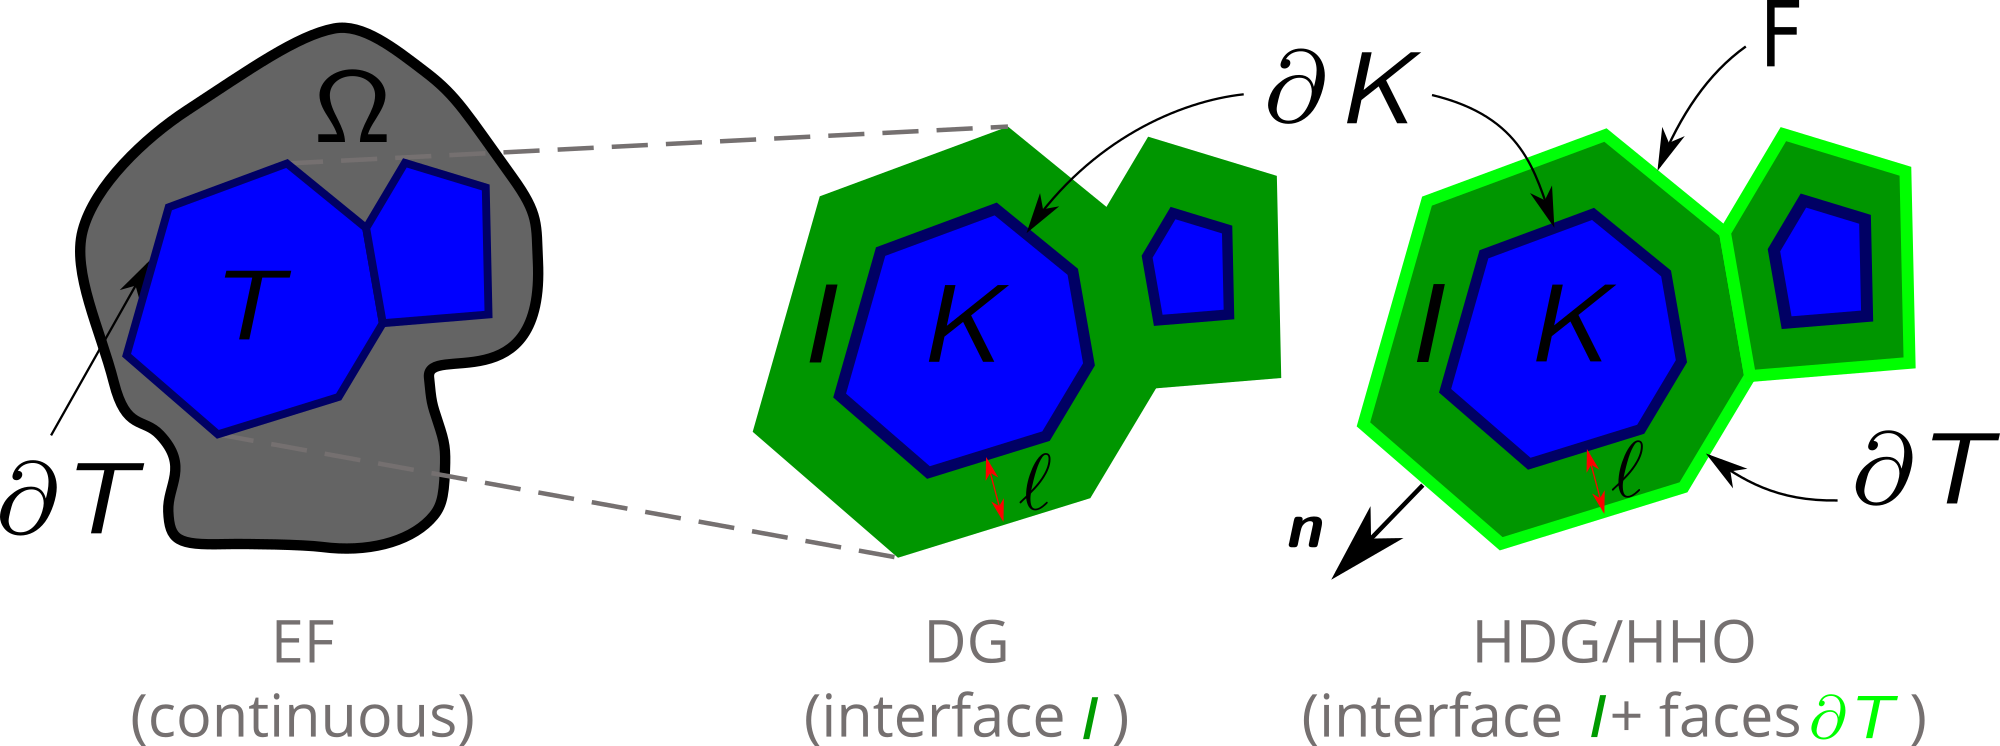
\includegraphics[width=14.cm]{img_calcs/ef_dg_hdg.png}
    \caption{schematic representation of a cell and its surrounding depending on the continuity requirement of the displacement field}
    \label{fig_02}
\end{figure}
%
%
%

% ---------------------------------------------------------
% PARAGRAPH
% ---------------------------------------------------------
\paragraph{Element behaviour}

The core of the element $\Bulk{}$ is made out of the same material that composes $\Omega$ and behaves according to the free energy potential $\mecPotential{}_{\bodyLag{}}$. The interface $\Crown{}$ is made out of a pseudo linear elastic material of Young modulus $\beta (\ell / h_{\cell})$ with a zero Poisson ratio and its behavior is defined by the free energy potential $\mecPotential{}_{\Crown{}}$ such that
%
%
%
\begin{equation}
    \label{eq_0009}
        \mecPotential{}_{\Crown} = \frac{1}{2} \beta \frac{\ell}{h_{\cell}} \nabla \tensori{u}{}_{\Crown} : \nabla \tensori{u}{}_{\Crown}
\end{equation}
%
%
%
where the dimensionless ratio $\ell / h_{\cell}$ balances the accumulated energy with the size of the domain $\cell$.

% ---------------------------------------------------------
% PARAGRAPH
% ---------------------------------------------------------
\paragraph{Element loading}

The core $\Bulk$ is subjected to the volumetric loading $\loadLag{}$, and to the traction force applied by the interface $\Crown{}$ onto $\dBulk{}$. By continuity, $\Bulk{}$ applies the opposite traction force on $\Crown{}$ through $\dBulk{}$. The interface $\Crown{}$ is also subjected to the exterior traction force $\neumannCellLoad{}$ acting on $\neumannCell{}$, that accounts for the action of the rest of the solid $\bodyLag{}$ onto the boundary $\dCell$.

% ---------------------------------------------------------
% PARAGRAPH
% ---------------------------------------------------------
\paragraph{Discplacement, displacement gradient and stress fields}

Let note $\tensori{u}{}_{\Bulk}$ the displacement field, $\tensorii{G}{}_{\Bulk}$ the displacement gradient field and $\tensorii{P}{}_{\Bulk}$ the stress field in $\Bulk{}$. Similarly, let $\tensori{u}{}_{\Crown{}}$ the displacement field, $\tensorii{G}{}_{\Crown}$ the displacement gradient field and $\tensorii{P}{}_{\Crown}$ the stress field in $\Crown{}$.
The displacement of the boundary $\dCell{}$ is denoted $\tensori{u}{}_{\dCell{}}$.
By continuity of the displacement field between $\Bulk{}$ and $\dCell$,  the displacement $\tensori{u}{}_{\Crown{}}$ verifies
%
% 
% 
\begin{subequations}
    \label{eq_conformity}
        \begin{alignat}{2}
        \tensori{u}{}_{\Crown} \vert_{\dBulk} & = \tensori{u}{}_{\Bulk} \vert_{\dBulk}
        \label{eq_conformity:eq1}
        \\
        \tensori{u}{}_{\Crown} \vert_{\dCell} & = \tensori{u}{}_{\dCell}
        \label{eq_conformity:eq2}
    \end{alignat}
\end{subequations}

% ---------------------------------------------------------
% PARAGRAPH
% ---------------------------------------------------------
\paragraph{Hu-Washizu Lagrangian of the element}

By combining both the Lagragian of the core $\Bulk{}$ and that of the interface $\Crown{}$, one obtains the total Lagragian $L_{\cell}^{HW}$ over the element such that
%
%
%
\begin{equation}
    \label{eq_hu_washizu_split}
    L_{\cell}^{HW}
    % (\tensori{u}{}_{\cell}, \tensorii{G}{}_{\cell}, \tensorii{P}{}_{\cell})
    =
    \int_{\Bulk} \mecPotential_{\bodyLag{}} + (\nabla \tensori{u}{}_{\Bulk} - \tensorii{G}{}_{\Bulk}) : \tensorii{P}{}_{\Bulk}
    +
    \int_{\Crown} \mecPotential_{\Crown{}} + (\nabla \tensori{u}{}_{\Crown} - \tensorii{G}{}_{\Crown}) : \tensorii{P}{}_{\Crown}
    -
    \int_{\Bulk} \loadLag \cdot \tensori{u}{}_{\Bulk}
    % -
    % \int_{\Crown} \loadLag \cdot \tensori{u}{}_{\Crown}
    -
    \int_{\neumannCell} \neumannCellLoad \cdot \tensori{u}{}_{\dCell}
\end{equation}

% ---------------------------------------------------------
% -- SUBSECTION
% ---------------------------------------------------------
\subsection{Hypotheses}
\label{sec_assumtions}

Since the interface is of negligible volume compared to that of the core, let make the following assumptions on the displacement and the stress fields in the interface.

% ---------------------------------------------------------
% PARAGRAPH
% ---------------------------------------------------------
\paragraph{Displacement in the interface}

The displacement in the interface $\Crown$ is assumed to be linear with respect to $\tensori{n}$, such that
its gradient is homogeneous in $\Crown{}$ along $\tensori{n}$
%
% 
% 
\begin{equation}
    \label{eq_crown_displacement}
    \nabla
    \tensori{u}{}_{\Crown}
    =
    \frac{\tensori{u}{}_{\dCell}
    -
    \tensori{u}{}_{\Bulk} \vert_{\dBulk} }{\ell} \otimes \tensori{n}
\end{equation}
% 
% 
%
That is, the displacement of the interface $\Crown{}$ linearly bridges that of the boundary $\dCell{}$ to that of the bulk $\Bulk{}$.

% ---------------------------------------------------------
% PARAGRAPH
% ---------------------------------------------------------
\paragraph{Stress in the interface}

Furthermore, let assume that $\tensorii{P}{}_{\Crown}$ is constant along the direction $\tensori{n}{}$ in $\Crown{}$. By continuity of the traction force across $\dBulk$, the following equality holds true
%
% 
% 
\begin{equation}
    \label{eq_continuity_traction_force}
    \begin{aligned}
        (\tensorii{P}{}_{\Crown} \vert_{\dBulk{}} - \tensorii{P}{}_{\Bulk} \vert_{\dBulk{}}) \cdot \tensori{n}{} = 0
        % &&
        % \text{in}
        % &&
        % \Crown{}
    \end{aligned}
\end{equation}

% ---------------------------------------------------------
% -- SUBSECTION
% ---------------------------------------------------------
\subsection{Towards Hybrid discontinuous methods from the Hu-Washizu Lagrangian}

Using the hypotheses stated in Section \ref{sec_assumtions} on the displacement field and the stress field in $\Crown{}$,
one can write \eqref{eq_hu_washizu_split} as a term depending on the thickness of the interface $\ell$ and on the core and boundary unknowns only. The reader can refer to \ref{sec_appendix_Hu_Washizu} for more details.

% ---------------------------------------------------------
% PARAGRAPH
% ---------------------------------------------------------
\paragraph{Simplified Hu–Washizu Lagrangian for a vanishing interface}

In particular, making the thickness of the interface $\ell \rightarrow 0$, such that $\Crown{}$ vanishes and the core part $\Bulk{}$ identifies to $\cell$, one obtains the simplified Hu–Washizu Lagrangian
% 
% 
%
\begin{equation}
    \label{eq_0015}
    \begin{aligned}
        L_{\cell}^{HW}
        = &
        \int_{\cell{}} \mecPotential{}_{\bodyLag{}} + (\nabla \tensori{u}{}_{\cell{}} - \tensorii{G}{}_{\cell{}}) : \tensorii{P}{}_{\cell}
        % \\
        % &
        + \int_{\dCell{}} (\tensori{u}{}_{\dCell} - \tensori{u}{}_{\cell} \vert_{\dCell}) \cdot \tensorii{P}{}_{\cell} \vert_{\dCell{}} \cdot \tensori{n}{}
        % \\
        % &
        + \int_{\dCell} \frac{\beta}{2 h_{\cell}} \lVert \tensori{u}{}_{\dCell{}} - \tensori{u}{}_{\cell{}} \vert_{\dCell{}} \rVert^2
        \\
        &
        -
        \int_{\cell} \loadLag{} \cdot \tensori{u}{}_{\cell{}}
        -
        \int_{\neumannCell{}} \neumannCellLoad{} \cdot \tensori{u}{}_{\dCell{}}
    \end{aligned}
\end{equation}
%
%
%
which fully defines the equilibrium of an element for discontinuous methods.

% ---------------------------------------------------------
% PARAGRAPH
% ---------------------------------------------------------
\paragraph{Hybridization of the primal unknown; the HDG and HHO methods}

Since the interface $\Crown{}$ has vanished by making $\ell \rightarrow 0$, both $\tensori{u}{}_{\cell} \vert_{\dCell{}}$ the trace of the displacement of the core part $\cell$ onto $\dCell{}$ and the displacement of the boundary $\tensori{u}{}_{\dCell{}}$ coexist on $\dCell{}$. The displacement of the element $\cell$ is thus said to be \textit{hybrid}, and is denoted by the pair $(\tensori{u}{}_{\cell}, \tensori{u}{}_{\dCell})$.

% ---------------------------------------------------------
% PARAGRAPH
% ---------------------------------------------------------
\paragraph{The special case of DG methods}

Replacing $\tensori{u}{}_{\dCell}$ by $\tensori{u}{}_{\cell'} \vert_{\dCell}$ for any neighboring cell $\cell'$ amounts to describe the framework of Discontinuous Galerkin methods, where only the core unknown $\tensori{u}{}_{\cell}$ is considered, and the displacement jump on $\dCell$ depends on $\tensori{u}{}_{\cell'} \vert_{\dCell}$ the trace of the displacement of neighboring cells instead.

% ---------------------------------------------------------
% PARAGRAPH
% ---------------------------------------------------------
\paragraph{Conformal Galerkin formulation}

By strongly enforcing continuity of the displacement across $\dCell{}$ such that $\tensori{u}_{\cell} \vert_{\dCell} = \tensori{u}_{\dCell}$, one recovers the Principle of Virtual Work \eqref{eq_HW_0}, which defines the framework of conformal methods.

% ---------------------------------------------------------
% PARAGRAPH
% ---------------------------------------------------------
\paragraph{Lagrangian variations}

By differentiation of the total Lagrangian \eqref{eq_0015} with respect to each variable of the problem, one obtains the weak equations
%
%
%
\begin{subequations}
    \label{eq_0017}
        \begin{alignat}{3}
            \frac{\partial L_{\cell}^{HW}}{\partial \tensori{u}{}_{\cell}} \delta \tensori{u}{}_{\cell}
            = & \int_{\cell} \tensorii{P}{}_{\cell} : \nabla \delta \tensori{u}{}_{\cell}
            -
            \int_{\cell} \tensori{f}{}_V \cdot \delta \tensori{u}{}_{\cell}
            -
            \int_{\dCell{}} \tensori{\theta}{}_{\cell} \cdot \delta \tensori{u}{}_{\cell} \vert_{\dCell}
            &&
            \ \ \ \ \ \ \ \ 
            &&
            \forall \delta \tensori{u}{}_{\cell}
            % \in \virtualDisplacementSpaceCell
        \label{eq_0017:eq0}
        \\
            \frac{\partial L_{\cell}^{HW}}{\partial \tensori{u}{}_{\dCell}} \delta \tensori{u}{}_{\dCell}
            = &
            \int_{\neumannCell} (\tensori{\theta}{}_{\cell} - \tensori{t}{}_{\neumannCell}) \cdot \delta \tensori{u}{}_{\dCell}
            &&
            \ \ \ \ \ \ \ \ 
            &&
            \forall \delta \tensori{u}{}_{\dCell}
            % \in \virtualDisplacementSpaceDCell
        \label{eq_0017:eq1}
        \\
            \frac{\partial L_{\cell}^{HW}}{\partial \tensorii{P}{}_{\cell}} \delta \tensorii{P}{}_{\cell}
            = & \int_{\cell} (\nabla \tensori{u}{}_{\cell} - \tensorii{G}{}_{\cell} ) : \delta \tensorii{P}{}_{\cell}
            +
            \int_{\dCell} (\tensori{u}{}_{\dCell} - \tensori{u}{}_{\cell} \vert_{\dCell}) \cdot \delta \tensorii{P}{}_{\cell} \vert_{\dCell} \cdot \tensori{n}{}
            &&
            \ \ \ \ \ \ \ \ 
            &&
            \forall \delta \tensorii{P}{}_{\cell}
            % \in \stressSpaceCell
        \label{eq_0017:eq3}
        \\
            \frac{\partial L_{\cell}^{HW}}{\partial \tensorii{G}{}_{\cell}} \delta \tensorii{G}{}_{\cell}
            = &
            \int_{\cell} (\frac{\partial \mecPotential_{\bodyLag}}{\partial \tensorii{G}{}_{\cell}} - \tensorii{P}{}_{\cell}) : \delta \tensorii{G}{}_{\cell}
            &&
            \ \ \ \ \ \ \ \ 
            &&
            \forall \delta \tensorii{G}{}_{\cell}
            % \in \gradSpaceCell
        \label{eq_0017:eq2}
    \end{alignat}
\end{subequations}
% 
% 
%
where we introduced the \textit{reconstructed traction force} $\tensori{\theta}{}_{\cell} = \tensorii{P}{}_{\cell} \vert_{\dCell} \cdot \tensori{n}{} + (\beta / h_{\cell}) \tensori{J}(\tensori{u}{}_{\cell}, \tensori{u}{}_{\dCell})$, with
$\tensori{J}(\tensori{u}{}_{\cell}, \tensori{u}{}_{\dCell}) = \tensori{u}{}_{\dCell} - \tensori{u}{}_{\cell} \vert_{\dCell}$ the jump function on the boundary $\dCell$.
Following discretization, multiple jump function choices are available. The reader can refer to Section \ref{sec_stabilization} for more details regarding implementation aspects.
In particular, \eqref{eq_0017:eq0} is the expression of the Principle of Virtual Work in $\cell$, where the \textit{reconstructed traction force} $\tensori{\theta}{}_{\cell}$ replaces the usual expression $\tensorii{P}{}_{\cell} \cdot \tensori{n}{}$ in the external contribution. \eqref{eq_0017:eq1} denotes a supplementary equation to the usual continuous problem as described in \eqref{eq_hu_washizu_derivative_0}, to account for the continuity of the flux $\tensori{\theta}{}_{\cell}$ across the cell boundary.
\eqref{eq_0017:eq2} accounts for the constitutive equation in a weak sense, and \eqref{eq_0017:eq3} defines the equation of an enhanced gradient field, that does not reduce to the projection of $\nabla \tensori{u}{}_{\cell}$ as in \eqref{eq_hu_washizu_derivative_0:eq3}, since it is enriched by a boundary component that depends on the displacement jump.
This feature is at the origin of the robustness of non-conformal methods to volumetric locking (see \ref{sec_appendix_gradient} for more details on this note).

% ---------------------------------------------------------
% -- SUBSECTION
% ---------------------------------------------------------
\subsection{Problem in primal form}
\label{sec_hdg_element_equilibrium}

% ---------------------------------------------------------
% PARAGRAPH
% ---------------------------------------------------------
\paragraph{Reconstructed gradient}

Since minimization of \eqref{eq_0017:eq3} defines a linear problem with any displacement pair $(\tensori{v}{}_{\cell}, \tensori{v}{}_{\dCell})$, one can eliminate \eqref{eq_0017:eq3} from the system \eqref{eq_0017}. The resulting equation defines the so-called \textit{reconstructed gradient} $\tensorii{G}{}_{\cell}(\tensori{v}{}_{\cell}, \tensori{v}{}_{\dCell})$ associated with any displacement pair $(\tensori{v}{}_{\cell}, \tensori{v}{}_{\dCell})$, that solves
%
%
%
\begin{equation}
    \label{eq_grad}
    \begin{aligned}
        \int_{\cell} \tensorii{G}{}_{\cell} : \tensorii{\tau}{}_{\cell}
        =
        \int_{\cell}  \nabla \tensori{v}{}_{\cell} : \tensorii{\tau}{}_{\cell}
        +
        \int_{\dCell} (\tensori{v}{}_{\dCell} - \tensori{v}{}_{\cell} \vert_{\dCell}) \cdot \tensorii{\tau}{}_{\cell} \vert_{\dCell} \cdot \tensori{n}{}
        &&
        \forall \tensorii{\tau}{}_{\cell}
        % \in \stressSpaceCell
    \end{aligned}
\end{equation}
%
%
%
where $\tensorii{\tau}{}_{\cell}$ denotes an arbitrary kinematically admissible stress field.

% -> expliquer que quand saut tend vers 0, on retrouve le projection normale
%  ordre du gradient -> dire que même ordre que approximation primale, renvoie aux annexes

% ---------------------------------------------------------
% PARAGRAPH
% ---------------------------------------------------------
\paragraph{Stress tensor}

Likewise, \eqref{eq_0017:eq2} is eliminated from \eqref{eq_0017} since it is linear with $\tensorii{G}{}_{\cell}$. Assuming in addition that the space of kinematically admissible stress fields is included in that of kinematically admissible displacement gradient fields, \eqref{eq_0017:eq2} holds in a strong sense such that
%
%
%
\begin{equation}
    \label{eq_stress}
    \begin{aligned}
        \tensorii{P}{}_{\cell} = \frac{\partial \mecPotential_{\bodyLag}}{\partial \tensorii{G}{}_{\cell}}
    \end{aligned}
\end{equation}

% ---------------------------------------------------------
% PARAGRAPH
% ---------------------------------------------------------
\paragraph{Lagrangian variations in primal form}

Using \eqref{eq_stress} and \eqref{eq_grad}, problem \eqref{eq_0017} depends on the displacement unknowns only such that the only remaining variations of the total Lagrangian \eqref{eq_0015} are those with respect to both displacement variables.
A new total Lagrangian $L_{\cell}^{HDG}$ arises from the simplified problem such that
%
%
%
\begin{equation}
    \label{eq_total_lagragian_bis}
    \begin{aligned}
        L_{\cell}^{HDG}
        = &
        \int_{\cell{}} \mecPotential_{\bodyLag}
        +
        \int_{\dCell} \frac{\beta}{2 h_{\cell}} \lVert \tensori{J}(\tensori{u}{}_{\cell{}}, \tensori{u}{}_{\dCell{}}) \rVert^2
        -
        \int_{\cell} \loadLag{} \cdot \tensori{u}{}_{\cell{}}
        -
        \int_{\neumannCell{}} \neumannCellLoad{} \cdot \tensori{u}{}_{\dCell{}}
    \end{aligned}
\end{equation}
%
%
%
with respective cell and boundary displacement variations:
\begin{subequations}
    \label{eq_final_problem}
        \begin{alignat}{3}
            \frac{\partial L_{\cell}^{HDG}}{\partial \tensori{u}{}_{\cell}} \delta \tensori{u}{}_{\cell}
            = & \int_{\cell} \tensorii{P}{}_{\cell} : \nabla \delta \tensori{u}{}_{\cell}
            -
            \int_{\cell} \tensori{f}{}_V \cdot \delta \tensori{u}{}_{\cell}
            -
            \int_{\dCell{}} \tensori{\theta}{}_{\cell} \cdot \delta \tensori{u}{}_{\cell} \vert_{\dCell}
            &&
            \ \ \ \ \ \ \ \ 
            &&
            \forall \delta \tensori{u}{}_{\cell}
            % \in \virtualDisplacementSpaceCell
        \label{eq_final_problem:eq0}
        \\
            \frac{\partial L_{\cell}^{HDG}}{\partial \tensori{u}{}_{\dCell}} \delta \tensori{u}{}_{\dCell}
            = &
            \int_{\neumannCell} (\tensori{\theta}{}_{\cell} - \tensori{t}{}_{\neumannCell}) \cdot \delta \tensori{u}{}_{\dCell}
            &&
            \ \ \ \ \ \ \ \ 
            % \in \virtualDisplacementSpaceDCell
        \label{eq_final_problem:eq1}
    \end{alignat}
\end{subequations}
where $\tensorii{P}{}_{\cell}$ is defined by \eqref{eq_stress} and
depends on $\tensorii{G}{}_{\cell}$ which solves \eqref{eq_grad}.


%%
%
%
% ---------------------------------------------------------
% ---- SECTION
% ---------------------------------------------------------
\section{Discretization}
\label{sec-discretization}

In this section, we describe the problem in discrete form ...

% ---------------------------------------------------------
% -- SUBSECTION
% ---------------------------------------------------------
\subsection{Spatial discretization}

% ---------------------------------------------------------
% PARAGRAPH
% ---------------------------------------------------------
\paragraph{Faces and skeleton of the mesh}

The boundary $\dCell{}$ of each element is decomposed in faces, such
that a face $F$ is a subset of $\bodyLag$, and either there are two
cells $\cell_F$ and $\cell_F'$ such that $F = \dCell_F \cap \dCell_F'$
($F$ is then an interior face), or there is a single cell $\cell_F$ such
that $F = \dCell_F \cap \partial \Omega$ ($F$ is then an exterior face).
Let $\dHybridMesh(\bodyLag) = \{ F_i \subset \bodyLag \ \vert \ 1 \leq i
\leq N_{F} \}$ the skeleton of the mesh, collecting all element faces
$F_i$ in the mesh, where $N_{F}$ denotes the number of faces. The set of
faces subjected to Neumann boundary conditions is denoted
$\dHybridMesh{}_{N}^e(\bodyLag)$, and $\dHybridMesh{}_{D}^e(\bodyLag)$
denotes that subjected to Dirichlet boundary conditions. Moreover, let
$\mathcal{F}^i(\bodyLag)$ the set of interior faces. For any cell
$\cell$, let $\mathcal{F}(\cell) = \{ F \in \dHybridMesh \ \vert \ F
\subset \dCell \}$ the set of faces composing the boundary of $\cell$,
and let $N_{\dCell}$ the number of faces in $\dCell$.

% ---------------------------------------------------------
% PARAGRAPH
% ---------------------------------------------------------
\paragraph{Mesh description}

Likewise, one defines the collection of all cells in the mesh
as $\HybridMesh(\bodyLag) = \{ \matI \subset \bodyLag \ \vert \ 1 \leq i
\leq N_{\cell} \}$, where $N_T$ denotes the total number of cells. The
composition of both $\mathcal{T}(\bodyLag)$ and
$\dHybridMesh{}(\bodyLag)$ forms the hybrid mesh
$\HybridMeshWhole({\bodyLag}) = \{ \mathcal{T}(\bodyLag),
\mathcal{F}(\bodyLag) \}$.

% ---------------------------------------------------------
% -- SUBSECTION
% ---------------------------------------------------------
\subsection{Functional discretization}

% ---------------------------------------------------------
% PARAGRAPH
% ---------------------------------------------------------
\paragraph{Discrete functional space}

For a cell $\cell$, we denote $\discreteDisplacementSpaceCell$ an
approximation space of finite dimension for the displacement in the
cell, and $V^h(F)$ that on a face $F \in \mathcal{F}(\cell)$. The
approximation space on $\dCell$ is $V^h(\dCell) = \prod_{F \in
  \mathcal{F}(\cell)} V^h(F)$. Similarly, let $\discreteGradSpaceCell$
the approximation space of the reconstructed gradient and
$\discreteStressSpaceCell$ that chosen for the stress.

\paragraph{Approximation bases. Local unknowns}

Let $\mathfrak{B}_T^h$ denote a basis of dimension $N_T^h$ in
$\discreteDisplacementSpaceCell$, and $\mathfrak{B}_F^h$ a basis of
dimension $N_F^h$ in $V^h(F)$. The specific choice of monomial bases for
$\mathfrak{B}_T^h$ and $\mathfrak{B}_F^h$ is discussed in depth in
\ref{sec_implementation}, though other bases can be chosen.

A function $\tensori{u}{}_{T}^h \in U^h(T)$ (respectively
$\tensori{u}{}_{F}^h \in V^h(F)$), is associated with vector of
coefficients $\mathfrak{U}_T$ of size $N_T^h$ (respectively
$\mathfrak{U}_F$ of size $N_F^h$).

\paragraph{Global Unknowns}

Let $(\tensori{u}{}_{\mathcal{T}}^h, \tensori{u}{}_{\mathcal{F}}^h)
\in U^h(\mathcal{T}) \times U^h(\mathcal{F})$ the global displacement
unknown of problem \eqref{eq_final_problem} in discrete form, where
$\tensori{u}{}_{\mathcal{T}}^h$ and $\tensori{u}{}_{\mathcal{F}}^h$ are
the piece-wise continuous displacements such that:
\begin{equation}
  \begin{aligned}
    \tensori{u}{}_{\mathcal{T}}^h
    \vert_{\cell} = \tensori{u}{}_{\cell}^h = \mathfrak{U}_T \cdot
    \mathfrak{B}_T^h && \forall \cell \in \mathcal{T} && \text{and} &&
    \tensori{u}{}_{\mathcal{F}}^h \vert_{F} = \tensori{u}{}_{F}^h =
    \mathfrak{U}_F \cdot \mathfrak{B}_F^h && \forall F \in \mathcal{F}
  \end{aligned}
\end{equation}
with $U^h(\mathcal{T}) = \prod_{T \in \mathcal{T}} U^h(T)$ and
$U^h(\mathcal{F}) = \prod_{F \in \mathcal{F}} U^h(F)$.

Likewise, let $\tensori{u}{}_{\dCell}^h \in V^h(\dCell)$ such
that $\tensori{u}{}_{\dCell}^h \vert_F = \tensori{u}{}_{F}^h, \forall F
\in \mathcal{F}(\partial T)$, where $V^h(\dCell) = \prod_{F \in
  \mathcal{F}(T)} U^h(F)$. In the following, let
$\mathfrak{U}_{\mathcal{T}}$ the unknown coefficient vector associated
to $\tensori{u}{}^h_{\mathcal{T}}$, $\mathfrak{U}_{\mathcal{F}}$ that to
$\tensori{u}{}^h_{\mathcal{F}}$, and $\mathfrak{U}_{\mathcal{\dCell}}$
that to $\tensori{u}{}^h_{\dCell}$.

% ---------------------------------------------------------
% -- SUBSECTION
% ---------------------------------------------------------
\subsection{Local and global discrete problems}

% ---------------------------------------------------------
% PARAGRAPH
% ---------------------------------------------------------
\subsubsection{Local residual}

In a functional space of finite dimension, the restriction of a linear
form can be represented a vector in the dual space. Hence, let
$\mathfrak{R}_{\cell}$ and $\mathfrak{R}_{\dCell}$ the residual vectors
associated with the the variations of the total
Lagrangian~\eqref{eq_0015}:
\begin{subequations}
  \label{eq_final_problem_00}
  \begin{alignat}{3}
    \mathfrak{R}_{\cell}(\mathfrak{U}_{\cell},
    \mathfrak{U}_{\dCell}) \cdot \mathfrak{\hat{U}}_{T}
    % \int_{\mathcal{T}} R_{\mathcal{T}}(\tensori{u}{}_{\mathcal{T}}, \tensori{u}{}_{\mathcal{F}}) \cdot \tensori{\hat{u}}{}_{\mathcal{T}}
 = & \int_{\cell} \tensorii{P}{}_{\cell}^h : \nabla
    \tensori{\hat{u}}{}_{\cell}^h - \int_{\cell} \tensori{f}{}_V \cdot
    \tensori{\hat{u}}{}_{\cell} - \int_{\dCell{}}
    \tensori{\theta}{}_{\cell}^h \cdot \tensori{\hat{u}}{}_{\cell}^h
    \vert_{\dCell} && \ \ \ \ \ \ \ \ && \forall
    \hat{\mathfrak{U}}_{\cell} % \in \virtualDisplacementSpaceCell
    \label{eq_final_problem_00:eq0} \\
    \mathfrak{R}_{\dCell}(\mathfrak{U}_{\cell},
    \mathfrak{U}_{\dCell}) \cdot \mathfrak{\hat{U}}_{\dCell}
    % \int_{\mathcal{F}} R_{\mathcal{F}}(\tensori{u}{}_{\mathcal{T}}, \tensori{u}{}_{\mathcal{F}}) \cdot \tensori{\hat{u}}{}_{\mathcal{F}}
 = & \int_{\dCell} (\tensori{\theta}{}_{\cell}^h -
    \tensori{t}{}_{\neumannCell}) \cdot \tensori{\hat{u}}{}_{\dCell}^h
    && \ \ \ \ \ \ \ \ && \forall \hat{\mathfrak{U}}_{\dCell}
    % \in \virtualDisplacementSpaceDCell \label{eq_final_problem_00:eq1}
    \label{eq_final_problem_00:eq1} \\
  \end{alignat}
\end{subequations}
where the discrete stress tensor $\tensorii{P}{}_{\cell}^h$ and the
discrete reconstructed gradient
$\tensorii{G}{}_{\cell}^h(\tensori{v}{}_{\cell}^h,
\tensori{v}{}_{\dCell}^h)$ are defined by the discrete forms of
equations \eqref{eq_stress} and \eqref{eq_grad} respectively such that:
\begin{equation}
  \label{eq_stress_discrete}
  \begin{aligned}
    \tensorii{P}{}_{\cell}^h =
    \frac{\partial \mecPotential_{\bodyLag}}{\partial
      \tensorii{G}{}_{\cell}^h} && \text{and} && \int_{\cell}
    \tensorii{G}{}_{\cell}^h : \tensorii{\tau}{}_{\cell}^h =
    \int_{\cell} \nabla \tensori{v}{}_{\cell}^h :
    \tensorii{\tau}{}_{\cell}^h + \int_{\dCell}
    (\tensori{v}{}_{\dCell}^h - \tensori{v}{}_{\cell}^h \vert_{\dCell})
    \cdot \tensorii{\tau}{}_{\cell}^h \vert_{\dCell} \cdot \tensori{n}{}
    && \forall \tensorii{\tau}{}_{\cell}^h \in S^h(\cell)
  \end{aligned}
\end{equation}
and the discrete reconstructed traction $\tensori{\theta}{}_{\cell}^h
= \tensorii{P}{}_{\cell}^h \cdot \tensori{n} + \beta / h_{\cell}
\tensori{J}^h(\tensori{v}{}_{\cell}^h, \tensori{v}{}_{\dCell}^h)$.

The solution of the discrete problem $(\mathfrak{U}_{\cell},
\mathfrak{U}_{\dCell})$ is defined by the fact that the associated
residuals $\mathfrak{R}_{\cell}$ and $\mathfrak{R}_{\dCell}$ must be
zero:
\begin{equation}
  \label{eq_final_problem_000}
  \begin{aligned}
    \mathfrak{R}_{\cell}(\mathfrak{U}_{\cell}, \mathfrak{U}_{\dCell})
    = 0 && \text{and} &&
    \mathfrak{R}_{\dCell}(\mathfrak{U}_{\cell}, \mathfrak{U}_{\dCell})
     = 0
  \end{aligned}
\end{equation}

In practice, the computation of $\mathfrak{R}_{\cell}$ and
$\mathfrak{R}_{\dCell}$ is discussed in depth in \ref{sec_implementation}.

% ---------------------------------------------------------
% PARAGRAPH
% ---------------------------------------------------------
\subsubsection{Global residuals and face assembly}

At the global scale, the solutions
$(\mathfrak{U}_{\mathcal{T}}, \mathfrak{U}_{\mathcal{F}})$ of the
discrete problem satisfies:
\begin{equation}
  \label{eq_final_global_problem_0}
  \begin{aligned}
    \forall \cell \in \mathcal{T}(\bodyLag), \forall
    \hat{\mathfrak{U}}_{\cell},
    \mathfrak{R}_{\cell}(\mathfrak{U}_{\cell}, \mathfrak{U}_{\dCell})
    \cdot \mathfrak{\hat{U}}_{T} & = 0 && \text{and} && \forall
    \hat{\mathfrak{U}}_{\mathcal{F}},
    \mathfrak{R}_{\mathcal{F}}(\mathfrak{U}_{\mathcal{T}},
    \mathfrak{U}_{\mathcal{F}}) \cdot \mathfrak{\hat{U}}_{\mathcal{F}} =
    0
  \end{aligned}
\end{equation}
where the vector
$\mathfrak{R}_{\mathcal{F}}(\mathfrak{U}_{\mathcal{T}},
\mathfrak{U}_{\mathcal{F}})$ is the skeleton residual such that~:
\begin{equation}
  \label{eq_final_problem_0}
  \begin{aligned}
    \mathfrak{R}_{\mathcal{F}}(\mathfrak{U}_{\mathcal{T}},
    \mathfrak{U}_{\mathcal{F}}) \cdot \mathfrak{\hat{U}}_{\mathcal{F}}
    % \int_{\mathcal{F}} R_{\mathcal{F}}(\tensori{u}{}_{\mathcal{T}}, \tensori{u}{}_{\mathcal{F}}) \cdot \tensori{\hat{u}}{}_{\mathcal{F}}
 = & \sum_{F \in \mathcal{F}^i(\bodyLag{})} \int_{F}
    (\tensori{\theta}{}_{\cell_F}^h + \tensori{\theta}{}_{\cell_F '}^h)
    \cdot \tensori{\hat{u}}{}_{F}^h + \sum_{F \in
      \mathcal{F}^e_N(\bodyLag{})} \int_{F}
    (\tensori{\theta}{}_{\cell_F}^h - \neumannLag) \cdot
    \tensori{\hat{u}}{}_{F}^h && \forall
    \hat{\mathfrak{U}}_{\mathcal{F}}
  \end{aligned}
\end{equation}

An interior face $F$ is linked to two adjacent cells $T$ and $T'$, and
each of these cells applies to the other a surface load $\pm
\tensori{t}{}_{T\cap T'}$ through $F$, which is identified with
$\tensori{t}{}_{\neumannCell\cap F}$ in \eqref{eq_final_problem_00:eq1}.
By summation over each face of the structure, these equal contributions
cancel out, which yields the expression of the first argument in the
right-hand side in \eqref{eq_final_problem_0}.

Since exterior faces subjected to Neumann boundary conditions are
linked to a single cell only, $\tensori{t}{}_{\neumannCell} =
\neumannLag$ on $\neumannBoundaryLag{}$, which yields the expression of
the second argument in the right-hand side in
\eqref{eq_final_problem_00:eq1}.

% ---------------------------------------------------------
% -- SUBSECTION
% ---------------------------------------------------------
\subsection{Cell unknowns elimination}

As the cell number of unknowns grows rapidly with the polynomial order
as compared to that in the face (See \ref{sec_shape_functions}), cell
unknowns must be eliminated for the for the method to be numerically
attractive.

In this section, two elimination strategies are examinated. The first
one, presented as the \textit{Cell equilibrium} strategy, has, to our
knowledge, never been introduced in the literature, and arises from the
previous total Lagrangian formulation of HDG methods. The second one
consists in performing a static condensation operation
\cite{abbas_hybrid_2018, abbas_hybrid_2019,di_pietro_hybrid_2015}
following linearization of the problem.

% ---------------------------------------------------------
% PARAGRAPH
% ---------------------------------------------------------
\subsubsection{Cell equilibrium}

This first algorithm considers that the cell displacement unknown
$\mathfrak{U}_{T}$ are defined as implicit functions of the boundary
displacement unknown $\mathfrak{U}_{\dCell}$ as follows:
\begin{equation}
  \label{eq_cell_equilibrium_1}
  \begin{aligned}
    \mathfrak{R}_{T}(\mathfrak{U}_{T}(\mathfrak{U}_{\dCell}),
    \mathfrak{U}_{\dCell}) = 0
  \end{aligned}
\end{equation}
In practice, Nonlinear Equation~\eqref{eq_cell_equilibrium_1} can be
solved by an iterative method. At the global scale, the face residual
can thus be expressed as function of the face displacement, and
satisfies:
\begin{equation}
  \label{eq_cell_equilibrium_face_residual}
  \mathfrak{R}_{\mathcal{F}}(\mathfrak{U}_{\mathcal{T}}\paren{\mathfrak{U}_{\mathcal{F}}},
 \mathfrak{U}_{\mathcal{F}})=0
\end{equation}

Nonlinear Equation~\eqref{eq_cell_equilibrium_face_residual} is
generally solved using an iterative method. For the sake of simplicity,
the Newton method is considered here. Let
\(\iter{n}{\mathfrak{U}_{\mathcal{F}}}\) be the current estimate of the
solution. The correction \(\iter{n}{\delta}\mathfrak{U}_{\mathcal{F}}\)
of this estimate is given by:
\[
\iter{n}{\delta}\mathfrak{U}_{\mathcal{F}}=
-\left( \frac{d\mathfrak{R}_{\mathcal{F}}}{d \mathfrak{U}_{\mathcal{F}}}
\right)^{-1} \,\cdot\,\iter{n}{\mathfrak{R}}_{\mathcal{F}}
\]
with
\(\iter{n}{\delta}\mathfrak{U}_{\mathcal{F}}=\iter{n+1}{\mathfrak{U}_{\mathcal{F}}}-\iter{n}{\mathfrak{U}_{\mathcal{F}}}\).


The jacobian matrix \(\frac{d\mathfrak{R}_{\mathcal{F}}}{d
  \mathfrak{U}_{\mathcal{F}}}\) can be determined using the chain rule,
as follows:
\begin{equation}
  \label{eq_cell_equilibrium_0}
  \begin{aligned}
    % R_{\mathcal{T}}(\mathfrak{U}_{\mathcal{T}})
    % \frac{d \mathfrak{R}_{\mathcal{F}}}{d \mathfrak{U}_{\mathcal{F}}}
    \frac{d\mathfrak{R}_{\mathcal{F}}}{d
      \mathfrak{U}_{\mathcal{F}}}
    = \frac{\partial
      \mathfrak{R}_{\mathcal{F}}}{\partial \mathfrak{U}_{\mathcal{T}}}
    \frac{\partial \mathfrak{U}_{\mathcal{T}}}{\partial
      \mathfrak{U}_{\mathcal{F}}} \cdot \delta
    \mathfrak{U}_{\mathcal{F}} + \frac{\partial
      \mathfrak{R}_{\mathcal{F}}}{\partial \mathfrak{U}_{\mathcal{F}}}
    \cdot \delta \mathfrak{U}_{\mathcal{F}}
  \end{aligned}
\end{equation}
Applying the implicit function theorem to
\eqref{eq_cell_equilibrium_1} yields:
\begin{equation}
  \label{eq_cell_equilibrium_2}
  \begin{aligned}
    \frac{\partial
      \mathfrak{U}_{\mathcal{T}}}{\partial \mathfrak{U}_{\mathcal{F}}} =
    - \frac{\partial \mathfrak{U}_{\mathcal{T}}}{\partial
      \mathfrak{R}_{\mathcal{T}}} \frac{\partial
      \mathfrak{R}_{\mathcal{T}}}{\partial \mathfrak{U}_{\mathcal{F}}}
  \end{aligned}
\end{equation}
Injecting \eqref{eq_cell_equilibrium_2} in
\eqref{eq_cell_equilibrium_0} yields the expression of the derivative of
the face resiudal with respect to the face displacement
\begin{equation}
  \label{eq_cell_equilibrium_3}
  \begin{aligned}
    % \frac{d \mathfrak{R}_{\mathcal{F}}}{d \mathfrak{U}_{\mathcal{F}}}
    \frac{d\mathfrak{R}_{\mathcal{F}}}{d
      \mathfrak{U}_{\mathcal{F}}} = \frac{\partial
      \mathfrak{R}_{\mathcal{T}}}{\partial \mathfrak{U}_{\mathcal{F}}}
    \cdot \delta \mathfrak{U}_{\mathcal{F}} - \frac{\partial
      \mathfrak{R}_{\mathcal{T}}}{\partial \mathfrak{U}_{\mathcal{T}}}
    \frac{\partial \mathfrak{U}_{\mathcal{T}}}{\partial
      \mathfrak{R}_{\mathcal{T}}} \frac{\partial
      \mathfrak{R}_{\mathcal{T}}}{\partial \mathfrak{U}_{\mathcal{F}}}
    \cdot \delta \mathfrak{U}_{\mathcal{F}}
  \end{aligned}
\end{equation}

% ---------------------------------------------------------
% PARAGRAPH
% ---------------------------------------------------------
\subsubsection{Static condensation}

In this section, $\mathfrak{U}_{\mathcal{T}}$ and
$\mathfrak{U}_{\mathcal{F}}$ are assumed to be independent variables.
Again, a Newton method is considered.

At the cell level, the correction of the cell unknown
$\iter{n}{\delta}\mathfrak{U}_{\cell}$ and face unknowns
$\iter{n}{\delta}\mathfrak{U}_{\dCell}$ are given by:
\begin{equation}
\label{eq_static_condensation_final}
\mathcal{K}\,\cdot\,
\begin{pmatrix}
  \iter{n}{\delta}\mathfrak{U}_{\cell}
  \\
  \iter{n}{\delta}\mathfrak{U}_{\dCell}
\end{pmatrix}
= -
\begin{pmatrix}
  \iter{n}{\mathfrak{R}}_{\mathcal{\cell}}
  \\
  \iter{n}{\mathfrak{R}}_{\mathcal{\dCell}}
\end{pmatrix}
\quad\text{with}\quad \mathcal{K} =
\begin{pmatrix}
  \derivtot{\mathfrak{R}_{\cell}}{\mathfrak{U}_{\cell}}
  & \derivtot{\mathfrak{R}_{\cell}}{\mathfrak{U}_{\dCell}} \\
  \derivtot{\mathfrak{R}_{\dCell}}{\mathfrak{U}_{\cell}}
  & \derivtot{\mathfrak{R}_{\dCell}}{\mathfrak{U}_{\dCell}} \\
\end{pmatrix}
=
\begin{pmatrix}
  \mathcal{K}_{\cell\cell} &
  \mathcal{K}_{\cell\dCell} \\
  \mathcal{K}_{\dCell\cell} &
  \mathcal{K}_{\dCell\dCell} \\
\end{pmatrix}
\end{equation}
where the blocks \(\mathcal{K}_{\cell\cell}\),
\(\mathcal{K}_{\cell\dCell}\), \(\mathcal{K}_{\dCell\cell}\) and
\(\mathcal{K}_{\dCell\dCell}\) have been introduced for convenience.

The correction of the cell unknown
$\iter{n}{\delta}\mathfrak{U}_{\cell}$ can thus be expressed as:
\begin{equation}
  \label{eq:cell_unknown_correction}
  \iter{n}{\delta}\mathfrak{U}_{\cell}=
  -\mathcal{K}_{\cell\cell}^{-1}\,\cdot\,\,\iter{n}{\mathfrak{R}}_{\mathcal{\cell}}
  -\mathcal{K}_{\cell\cell}^{-1}\,\cdot\,\mathcal{K}_{\cell\dCell}\,\cdot\,\iter{n}{\delta}\mathfrak{U}_{\dCell}
\end{equation}

The correction of the face unknown
$\iter{n}{\delta}\mathfrak{U}_{\dCell}$ satisfies:
\[
\paren{ \mathcal{K}_{\dCell\dCell}\,
  -\mathcal{K}_{\dCell\cell}\,\cdot\,\mathcal{K}_{\cell\cell}^{-1}\,\cdot\,\mathcal{K}_{\cell\dCell}
 }\,\cdot\, \iter{n}{\delta}\mathfrak{U}_{\dCell}=
-\iter{n}{\mathfrak{R}}_{\mathcal{\dCell}}
+\mathcal{K}_{\dCell\cell}\,\cdot\,\mathcal{K}_{\cell\cell}^{-1}\,\cdot\,\,\iter{n}{\mathfrak{R}}_{\mathcal{\cell}}
\]
or, introducing the condensed quantities
\(\iter{n}{\left.\mathfrak{R}^{c}_{\mathcal{\dCell}}\right.}\) and
\(\mathcal{K}_{\dCell\cell}^{c}\):
\[
\mathcal{K}_{\dCell\dCell}^{c}\,\cdot\,\iter{n}{\delta}\mathfrak{U}_{\dCell}=
-\iter{n}{\left.\mathfrak{R}^{c}_{\mathcal{\dCell}}\right.}
\]

The element contributions
\(\iter{n}{\left.\mathfrak{R}^{c}_{\mathcal{\dCell}}\right.}\) and
\(\mathcal{K}_{\dCell\cell}^{c}\) are then assembled to form the linear
system giving \(\iter{n}{\delta}\mathfrak{U}_{\mathcal{F}}\). Once,
\(\iter{n}{\delta}\mathfrak{U}_{\dCell}\) is known, a decondensation
step is performed to computed \(\iter{n}{\delta}\mathfrak{U}_{\cell}\)
using Equation~\ref{eq:cell_unknown_correction}.


\subsection{Extension to non linear materials with internal state variables}
\label{sec:discretization:extension_to_non_linear_materials}

This section is devoted to the extension of the method to non linear
materials with local internal state variables. Let \(\vec{Y}\) be the
set of internal state variables describing the material. Each cell is
assumed to describe a unique material.

To simplify the presentation and preseve a variational framework, the
behaviour of the material is assumed to be standard
generalized~\cite{moreau_sur_1970,halphen_sur_1975}. The evolution of
the material can thus be described by an incremental lagrangian
\(L_{\cell}^{HDG}\) defined as
follows~\cite{lorentz_variational_1999,forest_localization_2004}:
\begin{equation}
  L_{\cell}^{HDG} = \displaystyle \int_{\cell} \left[
  \mecPotential{}_{\bodyLag{}}+\Delta\,t\,\dissipationPotential\paren{\Frac{\vec{Y}^{\star}-\bts{\vec{Y}}}{\Delta\,t}}
 \right] + \int_{\dCell} \frac{\beta}{2 h_{\cell}} \lVert
  \tensori{J}(\tensori{u}{}_{\cell{}}, \tensori{u}{}_{\dCell{}})
  \rVert^2 - \int_{\cell} \loadLag{} \cdot \tensori{u}{}_{\cell{}} -
  \int_{\neumannCell{}} \neumannCellLoad{} \cdot
  \tensori{u}{}_{\dCell{}}
\end{equation}
where:
\begin{itemize}
  \item \(\dissipationPotential\) denotes the dissipation
  potential.
  \item \(\Delta\,t\) denotes the time increment.
  \item \(\bts{\vec{Y}}\) denotes the value of the internal state
  variables at the beginning of the time step.
\end{itemize}

At this stage, two strategies can be set-up to eliminate the internal
state variables:
\begin{enumerate}
  \item Classically, state variables are assumed to be defined at
  the integration points (or, expressed differently, to be approximated
  in \(L^{2}\)). This strategy is the one used by most finite element
  solvers. In pratice, given the increment of the reconstructed
  gradient, the constitutive equations, expressed as a system of
  ordinary differential equations, are integrated to compute the new
  value of the stress and the consistent tangent operator. This
  strategy, already used by Abbas et
  al.~\cite{abbas_hybrid_2018,abbas_hybrid_2019}, is used in the
  numerical examples of this paper.
  \item The state variables can also be approximated in some
  discrete space on the cell. In this case, the cell resolution
  algorithm could be extended to define the cell displacements and the
  state variables as implicit functions of the face displacements. This
  approach seems \emph{a priori} interesting in at least two cases:
  \begin{itemize}
    \item Applied to plasticity, this approach lead to a en
    potentially efficient multi-field
    plasticity~\cite{simo_computational_1998} method with a low
    computational cost as the extra degrees of freedoms (associated with
    the plastic strains) can be eliminated at the cell level.
    % Static condensation in the context of multi-field plasticty \cite{schroder_static_2015}.
    \item Applied to phase-field damage problems, the
    irreversibility constraint could be treated at the element level by
    defining appropriate Lagrange multiplier that can be eliminated. A
    similar idea was developped by Cicuttin et al. for the elliptic
    obstacle problem~\cite{cicuttin_hybrid_2020}.
  \end{itemize}
  Exploring those two lines of research is left for future
  works.
\end{enumerate}

%Moreover, it allows to consider extending the present cell correction
%iterative resolution to \textit{e.g.} constrained resolution algorithm,
%in order to solve inequality constrained problems, as encountered in
%multi-field plasticity~\cite{schroder_small_2015} for instance.

\subsubsection{Comparison between both schemes}
\label{par_cell_eq}

\paragraph{Static condensation}

The static condensation algorithm is the one used in the literature
\cite{di_pietro_discontinuous-skeletal_2015,cockburn_algorithm_2019,abbas_hybrid_2019-1,abbas_hybrid_2018}
to eliminate cell unknowns. Contrary to the introduced cell resolution
algorithm, this scheme needs not iterate at the cell level to accomodate
the cell correction. The actualization of the cell unknown displacement
by its correction requires that the quantities $\partial
\tensori{u}{}_{\cell}^l / \partial R_{\cell}^{\cell}$ and $\partial
R_{\cell}^{\cell} / \partial \tensori{u}{}_{\dCell}^k$ computed at the
previous iteration are known. From a numerical standpoint, this results
in keeping stiffness matrices blocks (see
Section~\ref{sec_implementation2}) in memory from an iteration to the
other.

\paragraph{Cell equilibrium}

The novel cell resolution scheme needs iterate at the cell level. It
may require to integrate the constitutive equation more times than the
static condensation algorithm does (See
paragraph~\ref{sec:discretization:extension_to_non_linear_materials}).
However, it allows to exactly evaluate the equilibrium of the cell with
its boundary, what does not the former.

\begin{figure}[H]
    \centering
    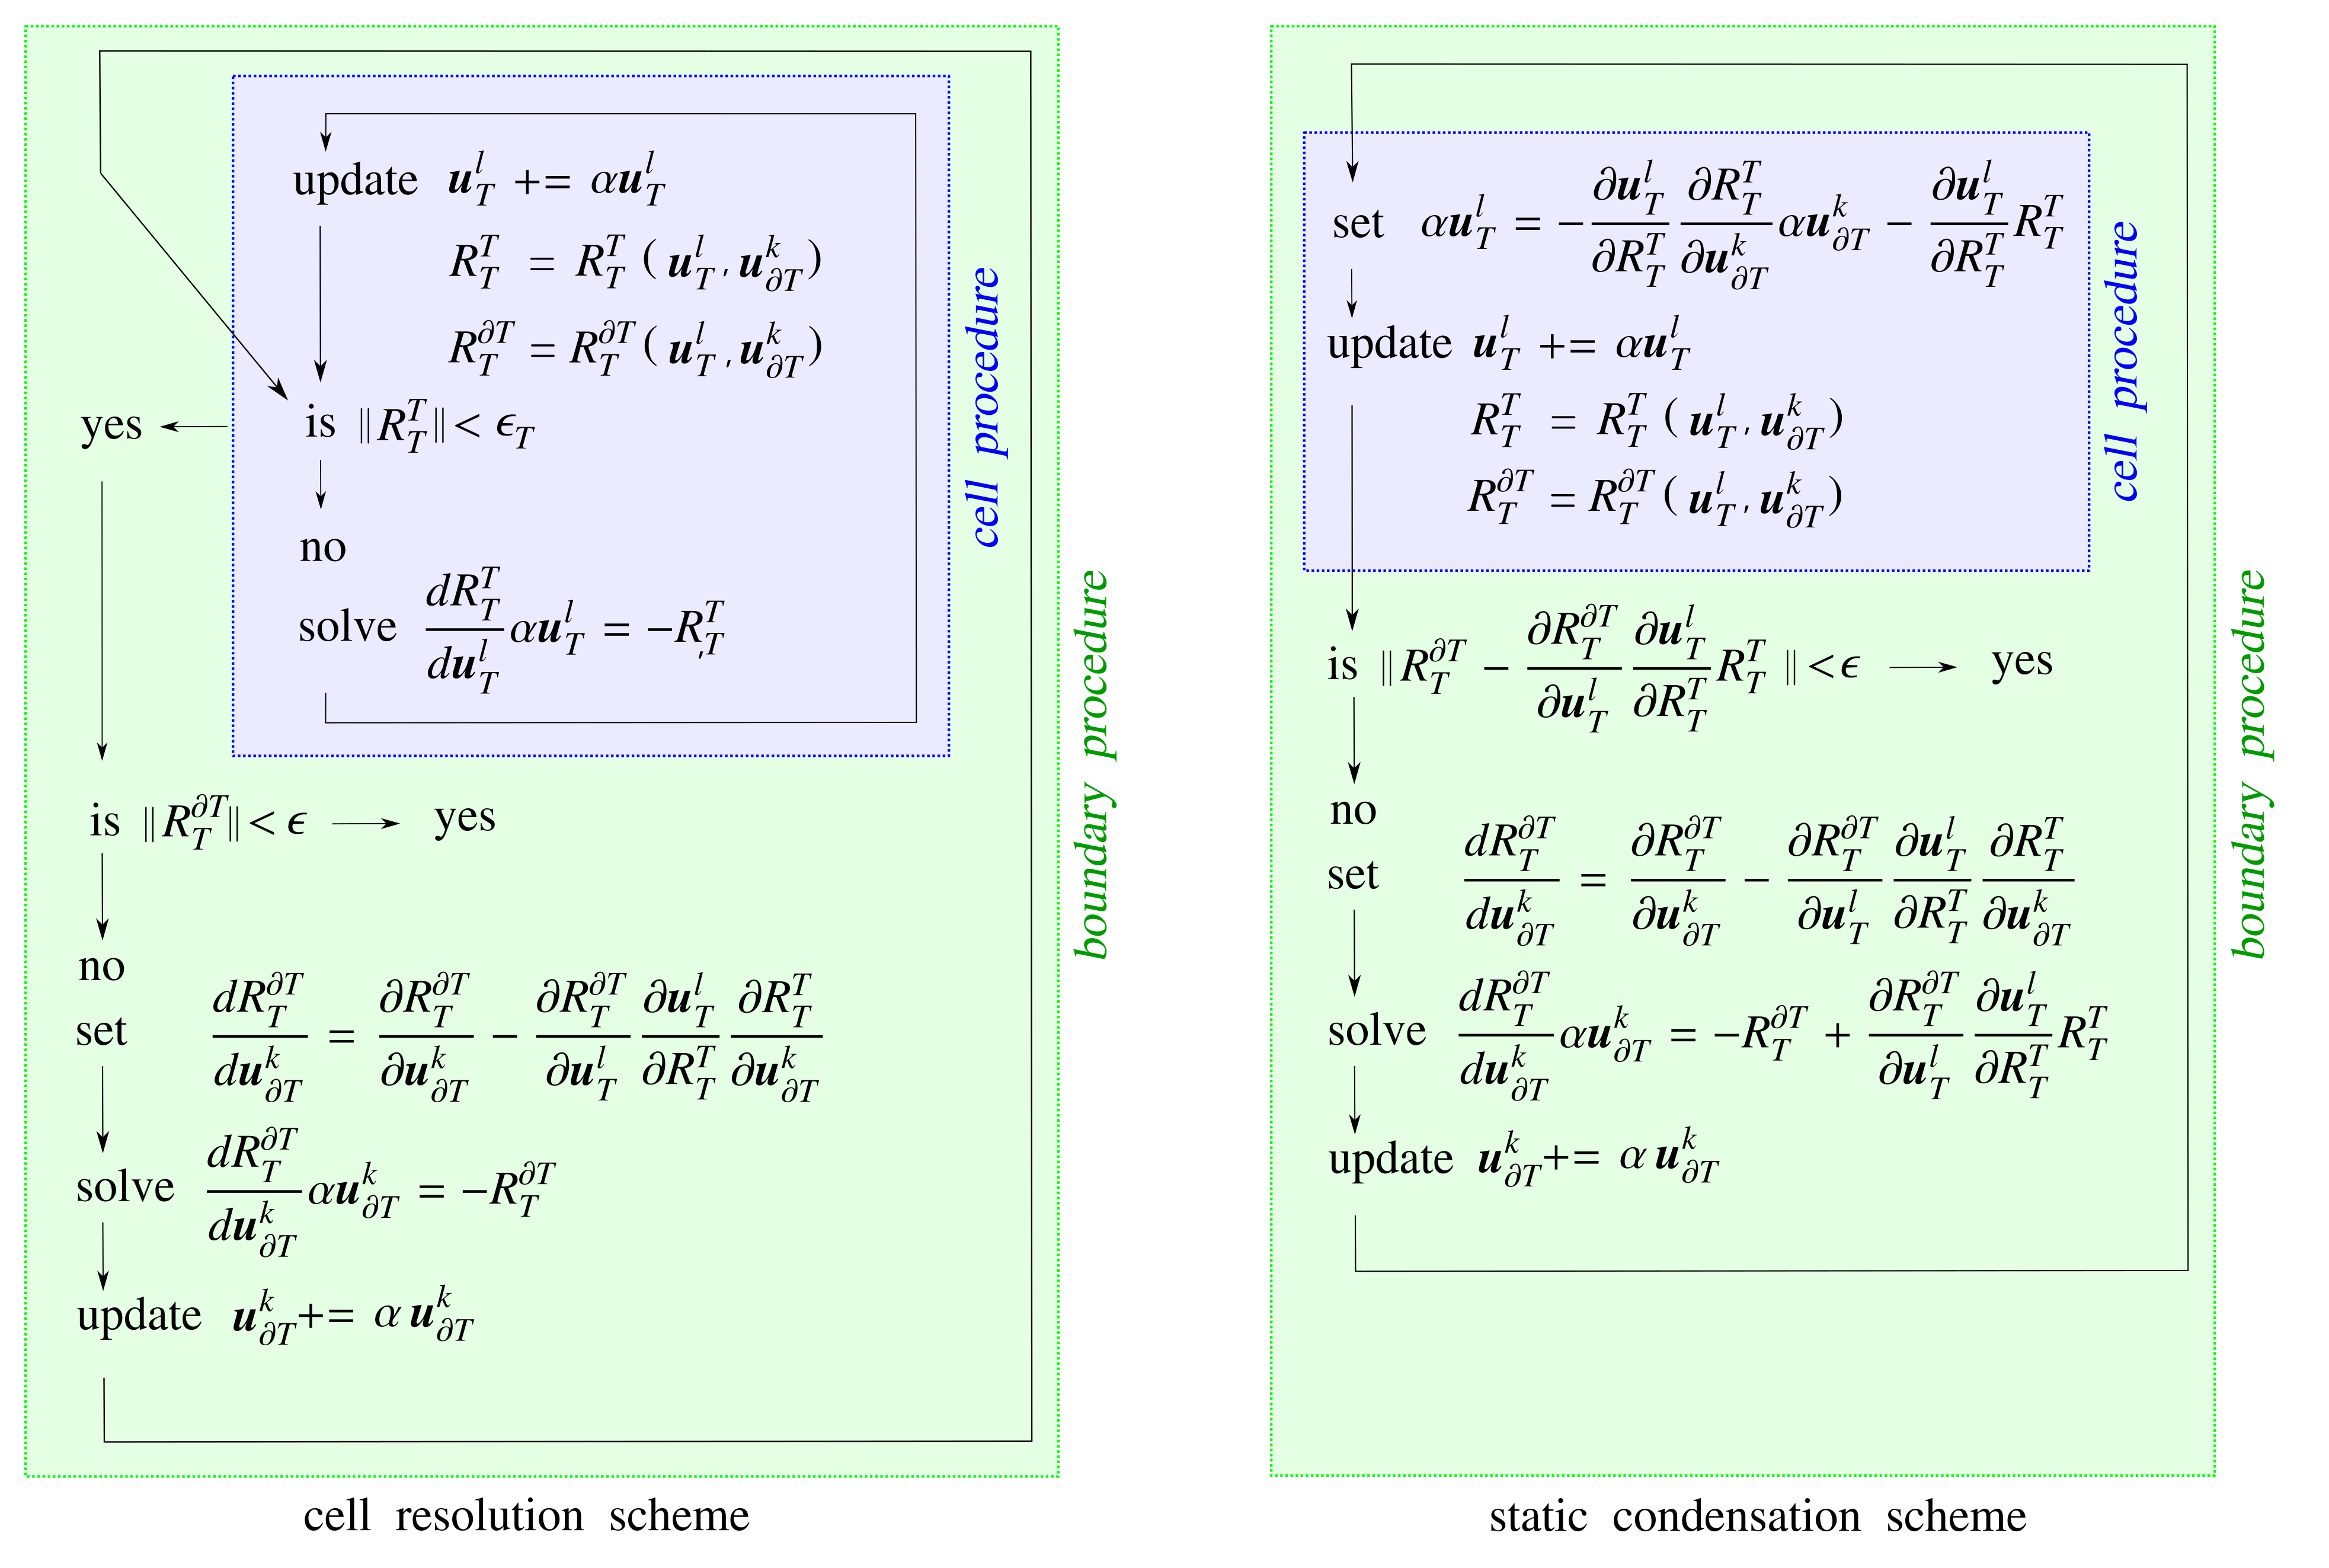
\includegraphics[width=15.cm]{img_calcs/resolution.png}
    \caption{Schematic representation of both resolution schemes}
    \label{fig_resolution}
\end{figure}


% NOTE : COMMENT ON TRACE LE DEPLACREMENT -> MOYENNE AU NOEUDS A PRECISER DANS LA LEGENDE DE LA FIGURE
% NOTE : LE CODE, CE QU'ON UTILISE, MFRONT MGIS -> IMPLEMENTATION PORTEE DANS CAST3M -> IMPLEMENTATION PLUGGABLE DANS AUTRE CHOSE -> 
% NOTE : ON PARLE PAS DES TEMPS DE CALCULS DANS LA SUITE parce que c du python, on montr que les 2 schémas d'intégration convergecne de manière qudartique, localement et globalement
% POUR ETRE COHERENT EN CONDENSATION, IL FAUT ACCLERER LES FACES +  LES CELLULES. POUR NOUS C QUE LES FACES


% ---------------------------------------------------------
% ---- SECTION
% ---------------------------------------------------------
\section{Numerical examples in the axisymmetric modelling hypothesis}
\label{sec_numerical_examples}

In this section, we evaluate the proposed axi-symmetric HHO method on
classical test cases taken from the literature to emphasize robustness
to volumetric locking. We consider both the small and large strains
framework, for elasto-plastic behaviors. In this section, we denote by
HHO($k,l$) the HHO element of order $k$ on faces, and order $l$ in the
cell.

The tests presented in this section have been performed using an
\texttt{python} implementation freely available on github: \url{...}.
The results of this implementations were toroughly compared to the
results obtained with the reference implementation provided the
\texttt{Disk++} solver.

% ---------------------------------------------------------
% PARAGRAPH
% ---------------------------------------------------------
\paragraph{Stabilization parameter}

To ensure coercivity of the HHO method, the stabilization parameter
$\beta$ needs be chosen according to the material under study. In the
literature~\cite{di_pietro_discontinuous-skeletal_2015}, a value of
order $2 \mu$ is advocated, where $\mu$ denotes the shear modulus of the
material. We use this values for all test cases in the present section.

% ---------------------------------------------------------
% -- SUBSECTION
% ---------------------------------------------------------
\subsection{The free dilatation test}
\label{sec_satoh_test}

The first test case of the following benchmark aims at displaying the
robustness of the HHO method for coupled mechanical-thermal problems.

% ---------------------------------------------------------
% PARAGRAPH
% ---------------------------------------------------------
\paragraph{Specimen and loading}

For this test case, the unit box is fixed on both the right and
bottom boundaries in their respective normal directions, and a quadratic
thermal load depending on the $r$-coordinate is imposed in the solid
(see Figure \ref{fig_satoh_setting}). The mesh is composed of 400
quadrangles. The thermal loading is given by:
%
%
%
\begin{equation}
    T(r,z) = 4 (T_{max} - T_{min})r(1 - r) + T_{min}
\end{equation}
%
%
%
with temperature values $T_{max} = 2000$ K and $T_{min} = 293.15$ K.

\begin{figure}[H]
    \centering
    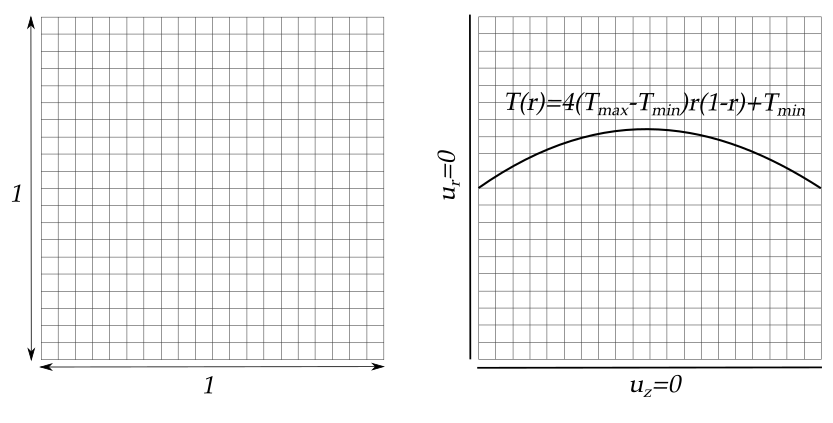
\includegraphics[width=10.cm]{img_calcs/satoh_setting.png}
    \caption{Geometry, displacement boundary conditions and temperature loading for the free dilatation test case}
    \label{fig_satoh_setting}
\end{figure}

% ---------------------------------------------------------
% PARAGRAPH
% ---------------------------------------------------------
\paragraph{Material behaviour}

A linear thermo-elastic energy potential is considered with a Young's
modulus $E$ equal to $150$ GPa. The material is quasi-incompressible
with a Poisson's ratio $\nu$ equal to $0.499$. The dilatation parameter
is taken as $\alpha = 1e^{-6}$ K$^{-1}$.

% ---------------------------------------------------------
% PARAGRAPH
% ---------------------------------------------------------
\paragraph{Volumetric locking and polynomial approximation for the strain and temperature fields}

Lagrange finite elements of order $1 \leq k \leq 2$ evaluate a
mechanical strain of order $0 \leq k-1 \leq 1$, whereas the thermal
strain is of order $2$. Using the total strain for the computation of
the stress results in strong volumetric locking. Hence, for Lagrange
element to accurately model the problem, one needs to choose a
temperature fields that is one order lower than that describing the
displacement field. This feature is of major importance for mixed
elements, where quadratic elements needs be employed to match the the
linear pressure unknown polynomial order.

\begin{figure}[H]
    \centering
    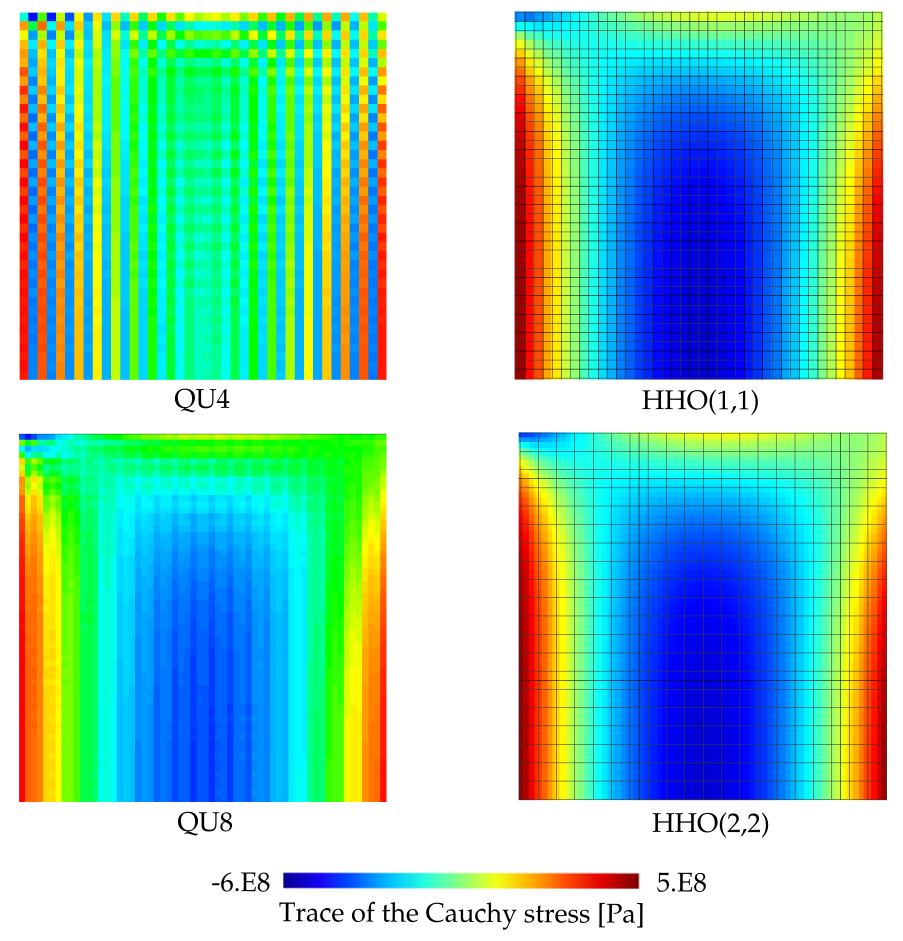
\includegraphics[width=10.cm]{img_calcs/satoh_calc.png}
    \caption{Map fo the Trace of the Cauchy stress at quadrature points for the Free dilatation test case at the last time step}
    \label{fig_satoh_calc}
\end{figure}

% ---------------------------------------------------------
% PARAGRAPH
% ---------------------------------------------------------
\paragraph{Comparison of FE and HHO methods}

In Figure \ref{fig_satoh_calc}, one can observe that the pressure map is completely smooth for the HHO computations, even for a quadratic temperature field acting on a linear gradient using HHO(1,1). As expected, the results display mild signs of volumetric locking for the quadratic finite element
approximation, and strong oscillations are noted for the linear finite element solution.

% ---------------------------------------------------------
% -- SUBSECTION
% ---------------------------------------------------------
\subsection{Perfect plastic swelling sphere}
\label{sec_swelling_sphere}

% ---------------------------------------------------------
% PARAGRAPH
% ---------------------------------------------------------
\paragraph{Specimen and loading}

This benchmark consists in a quasi-incompressible sphere under uniform internal loading.
This test case has an analytical solution and the state of the specimen is known when the plastic region has reached the external border of the sphere.
The sphere has an inner radius $r_{int} = 0.8$ mm and an outer
radius $r_{ext} = 1$ mm. An internal radial displacement $u$ is imposed. The mesh is composed of XXX quadrangles (see Figure \ref{fig_sphereall}).
The simulation is performed until the limit load corresponding to an internal displacement of $0.2$ mm is reached.

% ---------------------------------------------------------
% PARAGRAPH
% ---------------------------------------------------------
\paragraph{Material behaviour}

An isotropic hardening energy potential $\mecPotential{}_{\bodyLag{}}^p$ is chosen for the description of the plastic evolution of the material such that

\begin{equation}
    \mecPotential{}_{\bodyLag{}}^p(p)
    =
    \sigma_0 p + \frac{1}{2} H p^2 + (\sigma_{\infty} - \sigma_0)(p - \frac{1 - e^{-\delta p}}{\delta})
\end{equation}
%
%
%
where the parameter $p$ denotes the equivalent plastic strain and a Von Mises yields function $f$ describes the flow rule
%
%
%
\begin{equation}
    f = \sqrt{\frac{3}{2}} \rVert \text{dev} (\tensorii{\sigma}) \lVert - p
\end{equation}
%
%
%
Moreover, the small strain hypothesis is assumed for this test case.
Perfect plasticity is considered for this test case , where the saturation parameter $\delta = 0$, the yield stresses $\sigma_0 = \sigma_{\infty} = 6$ MPa, the hardening parameter $H = 0$ and the elastic potential parameters are the Young modulus $E = 28.85$ MPa and the Poisson ratio $\nu = 0.499$, such that the material is quasi-incompressible.

\begin{figure}[H]
    \centering
    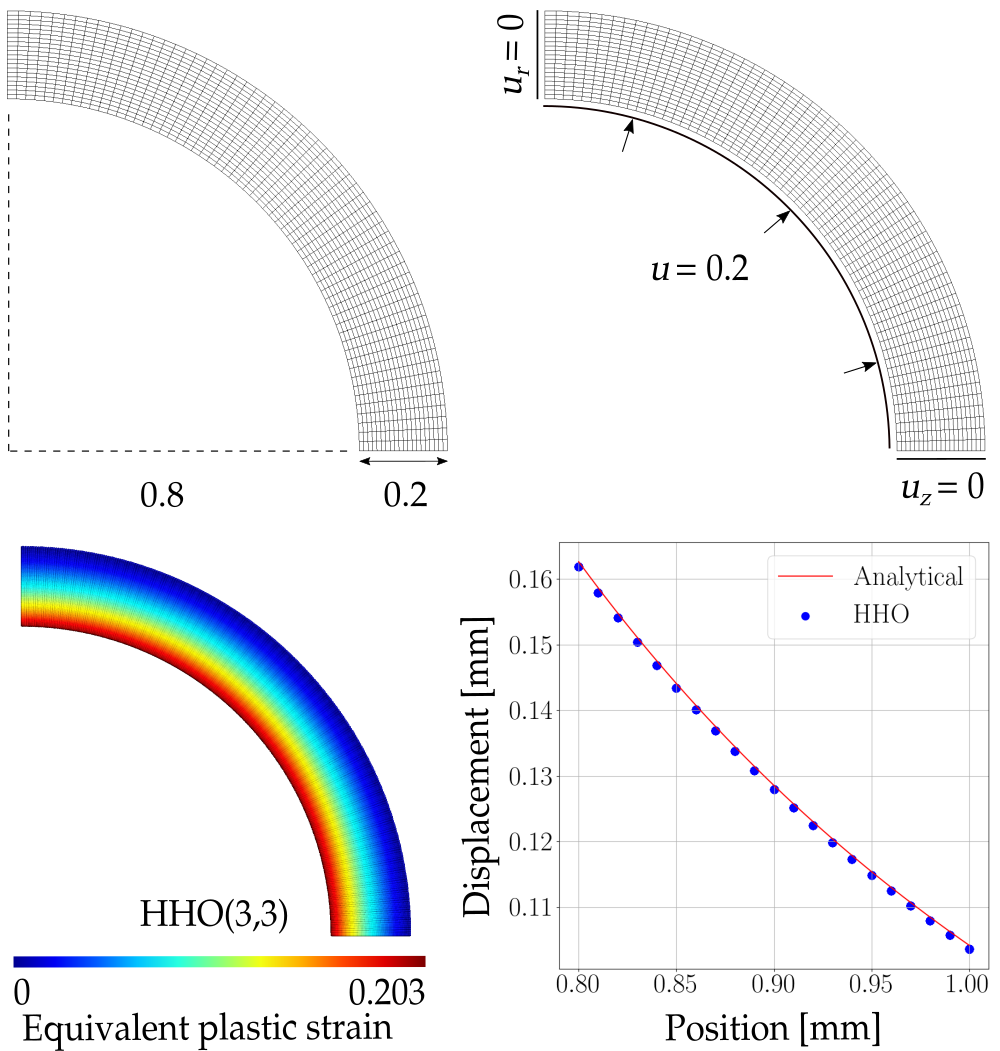
\includegraphics[width=12.cm]{img_calcs/sphere_mesh.png}
    \caption{the swelling sphere test case. Geometry, loadings, final displacement along the radius of the sphere, and final equivalent plastic strain map at quadrature points}
    \label{fig_sphereall}
\end{figure}

% ---------------------------------------------------------
% PARAGRAPH
% ---------------------------------------------------------
\paragraph{Displacement along the radius}

Since an analytical solution is known for this test case, we compare it to the proposed HHO method. The displacement of the section of the sphere at cell nodes
is plotted in Figure \ref{fig_sphereall}, along with the analytical one, and we observe that the obtained results are in agreement with the analytical response.
Figure \ref{fig_sphereall} mentions the label HHO without specifying approximation orders for all computations deliver the same result.

% ---------------------------------------------------------
% PARAGRAPH
% ---------------------------------------------------------
\paragraph{Trace of the Cauchy stress}

As for the displacement, the analytical solution for the trace of the Cauchy stress tensor is compared to the one computed using the proposed HHO method for three approximation orders.
A sign of volumetric locking is the presence of strong oscillations in the trace of the Cauchy stress (or, equivalently, the hydrostatic pressure) within elements.
We observe that numerical results at quadrature points fit the analytical curve, and display no sign of volumetric locking. The computed solution is however less smooth
at the borders of the specimen for higher orders, a phenomenon that was pointed out in \cite{abbas_hybrid_2019-1} for the three dimensional case, and attributed to the fact that planar faces are considered.

\begin{figure}[H]
    \centering
    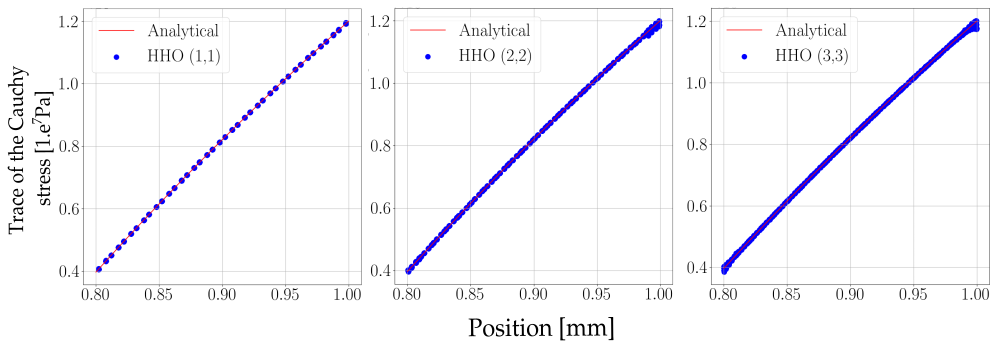
\includegraphics[width=15.cm]{img_calcs/sphere_pressures.png}
    \caption{trace of the Cauchy stress tensor along the radius of the sphere at quadrature points}
    \label{fig_sphere_pressure}
\end{figure}

% ---------------------------------------------------------
% -- SUBSECTION
% ---------------------------------------------------------
\subsection{Necking of a notched bar}

% ---------------------------------------------------------
% PARAGRAPH
% ---------------------------------------------------------
\paragraph{Specimen and loading}

We consider a notched bar that is subjected to uniaxial
extension.
The bar has a length of $30$ mm, a top section of radius $5$ mm and a bottom section of radius $3$ mm.
A vertical
displacement $u_z = 0.8$ mm is imposed at the top, as shown in Figure \ref{fig_ssnaallmesh}.
For symmetry reasons, only one-quarter of the
bar is discretized, and the mesh is composed of XXX quadrangles.

% ---------------------------------------------------------
% PARAGRAPH
% ---------------------------------------------------------
\paragraph{Behaviour law}

The same behavior law as that in \ref{sec_swelling_sphere} is considered for the present test case. 
However, the finite strain hypothesis is chosen, based on a logarithmic decomposition of the stress \cite{miehe_anisotropic_2002}.

% ---------------------------------------------------------
% PARAGRAPH
% ---------------------------------------------------------
\paragraph{Material parameters}

Materials parameters are taken as
$\sigma_0 = 450$ MPa, $\sigma_{\infty} = 715$ MPa with a saturation parameter $\delta = 16.93$. The Young modulus is $E = 206.9$ GPa, and the Poisson ratio is $\nu = 0.29$.

% ---------------------------------------------------------
% PARAGRAPH
% ---------------------------------------------------------
\paragraph{Load deflection curve}

The load-displacement curve is plotted
in Figure \ref{fig_ssnaallmesh}, and gives similar results to that obtained with quadratic reduced integration elements.

% ---------------------------------------------------------
% PARAGRAPH
% ---------------------------------------------------------
\paragraph{Equivalent plastic strain}

Moreover, the equivalent
plastic strain $p$ at quadrature points and at the final load is plotted Figure \ref{fig_ssnaallplastic}.
It has been observed that the equivalent plastic strain might suffer some oscillations at a certain limit load with UPG methods.
One notices through the present example, that the proposed HHO method displays no oscillations of the equivalent plastic strain.

\begin{figure}[H]
    \centering
    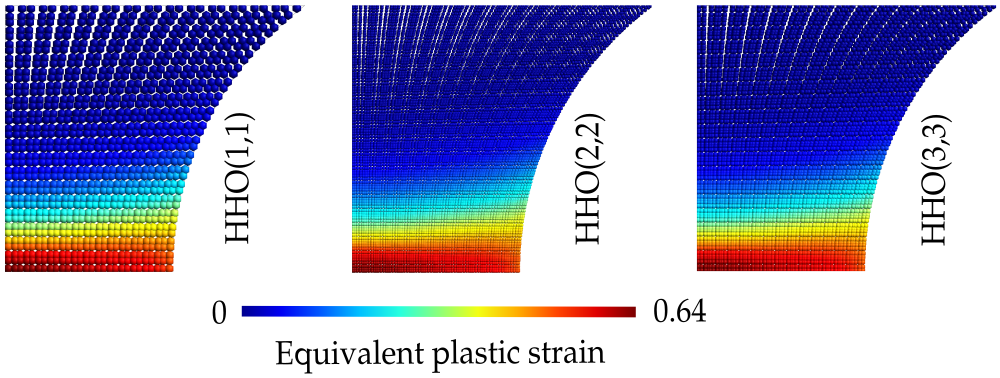
\includegraphics[width=12.cm]{img_calcs/ssna_plastic.png}
    \caption{
        final equivalent plastic strain map at quadrature points in the notch region
    }
    \label{fig_ssnaallplastic}
\end{figure}

% ---------------------------------------------------------
% PARAGRAPH
% ---------------------------------------------------------
\paragraph{Hydrostatic pressure}

The hyrostatic pressure map at quadrature points and at the final load is shown Figure \ref{fig_ssnaallmesh} for three HHO element orders (respectively $1, 2$ and $3$).
As for the swelling sphere test case, one notices that the hydrostatic pressure map is
fairly smooth over the whole structure at all approximation orders, even at the bottom left corner where plasticity is confined.

\begin{figure}[H]
    \centering
    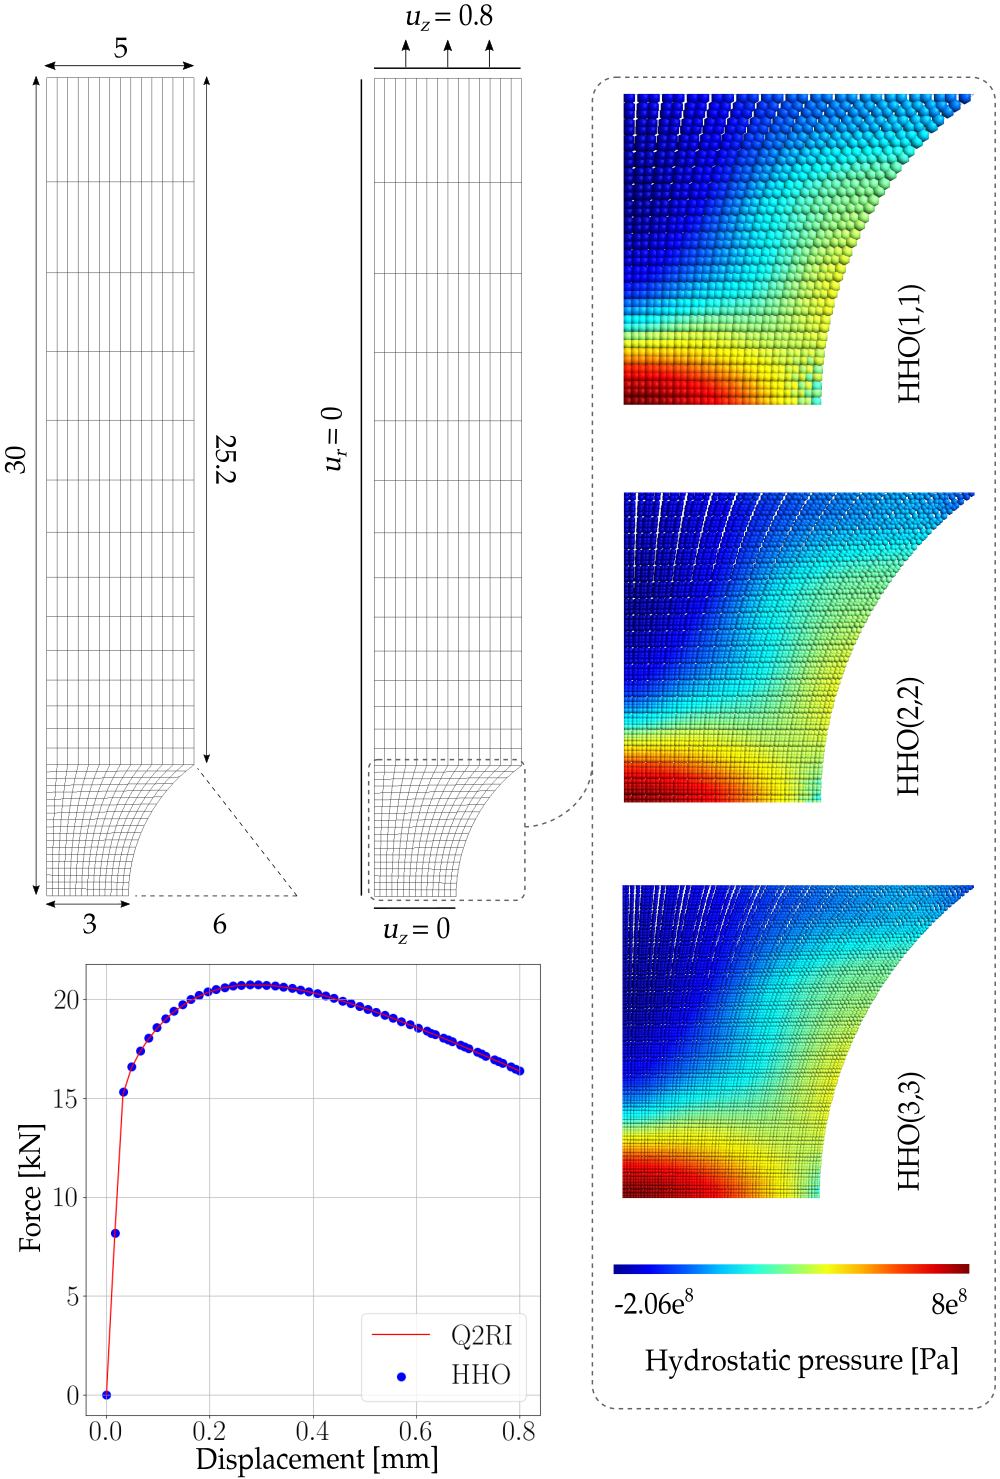
\includegraphics[width=12.cm]{img_calcs/ssna_mesh.png}
    \caption{
        the notched specimen test case. Geometry, loadings, load deflection curve, and final hydrostatic pressure map at quadrature points in the notch region
    }
    \label{fig_ssnaallmesh}
\end{figure}

% ---------------------------------------------------------
% ---- SECTION
% ---------------------------------------------------------
\section{Numerical examples in plane strain and tridimensional modelling hypotheses}
\label{sec_num_example_part_2}

The section showcases numerical examples demonstrating the robustness
of the cell resolution algorithm. The test cases under study, namely the
classical Cook membrane, and the indentation test cases, show that no
volumetric locking is encountered using the cell resolution algorithm.

% ---------------------------------------------------------
% -- SUBSECTION
% ---------------------------------------------------------
\subsection{Cook's membrane test case}

% ---------------------------------------------------------
% PARAGRAPH
% ---------------------------------------------------------
\paragraph{Specimen and loading}

Let consider the Cook membrane specimen that is subjected to uniaxial
traction. The membrane has a width of $48$ mm and a height of $60$ mm,
and a vertical traction $t_y = 1000$ N/m is imposed at the top. The HHO
computation is run on a polygonal mesh (see Figure \ref{fig_cook}) and
is compared with standard QU4 and QU8 formulations (\textit{i.e.} linear
and quadratic approximations)

% ---------------------------------------------------------
% PARAGRAPH
% ---------------------------------------------------------
\paragraph{Constitutive equation}

The same behavior law as that in \ref{sec_swelling_sphere} is
considered for the present test case. However, the finite strain
hypothesis is chosen, based on a logarithmic decomposition of the stress
\cite{miehe_anisotropic_2002}.

% ---------------------------------------------------------
% PARAGRAPH
% ---------------------------------------------------------
\paragraph{Material parameters}

Materials parameters are taken as
$\sigma_0 = 450$ MPa, $\sigma_{\infty} = 715$ MPa with a saturation parameter $\delta = 16.93$. The Young modulus is $E = 206.9$ GPa, and the Poisson ratio is $\nu = 0.29$.

\begin{figure}[H]
    \centering
    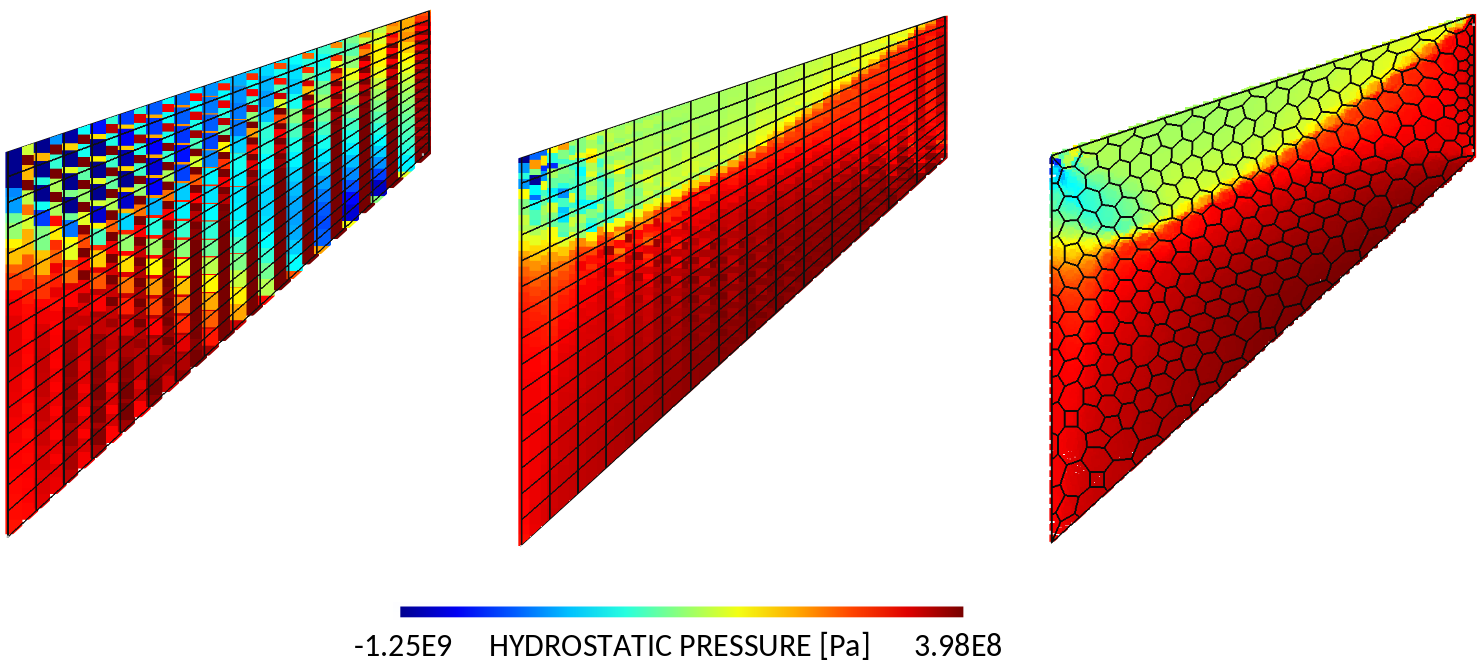
\includegraphics[width=12.cm]{img_calcs/cook_comp.png}
    \caption{Hydrostatic pressure map one the reference configuration at the limit load}
    \label{fig_cook}
\end{figure}

% ---------------------------------------------------------
% PARAGRAPH
% ---------------------------------------------------------
\paragraph{Numerical results}

As expected, the linear and quadratic finite element methods display respectively strong and mild oscillations of the pressure, whereas the HHO one shows no sign of locking.

% ---------------------------------------------------------
% -- SUBSECTION
% ---------------------------------------------------------
\subsection{Indentation test case}

% ---------------------------------------------------------
% PARAGRAPH
% ---------------------------------------------------------
\paragraph{Specimen and loading}

The last test case consists in the indentation of a cube of size $10$ mm. A pressure of $300$ MPa is imposed on the top surface see Figure \ref{fig_cube}).

% ---------------------------------------------------------
% PARAGRAPH
% ---------------------------------------------------------
\paragraph{Material}

The same perfect plastic material as that in \ref{sec_swelling_sphere} is considered for the present test case.

\begin{figure}[H]
    \centering
    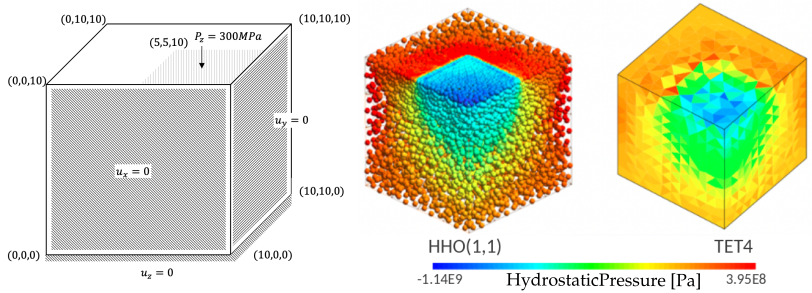
\includegraphics[width=12.cm]{img_calcs/cube.png}
    \caption{Hydrostatic pressure map one the reference configuration at the limit load}
    \label{fig_cube}
\end{figure}

% ---------------------------------------------------------
% PARAGRAPH
% ---------------------------------------------------------
\paragraph{Numerical results}

The pressure map at the end of the computation is displayed in Figure \ref{fig_cube}, and no sign of volumetric locking are present on the HHO computation, as opposed to the linear finite element one.

% ---------------------------------------------------------
% ---- SECTION
% ---------------------------------------------------------
\section{Conclusion}

% Dire de maniere explicte, mettre les éléments virtuels dans le même cadre -> dire quil reste à examiner le lien avec les éléments viertuels 
% Le HW permet de retrouver les principes HDG, HHO qui sont au coeur de ce paprier mais aussi les cG
% les VEM notn pas ete bconsideres, bien que le cadrez propos semblke sadapter à leur formalmisme
% descxirption du code, trouvaable sur github, avec chaque exemple

An introduction to HDG and HHO methods has been proposed, based on the minimization of a Hu-Washizu Lagrangian. The expression of the method arising from this approach allows to introduce naturally all the ingredients of the method, as well as the displacement discontinuity, in a unified framework.
This new formulation also allows one to draw a connection between HDG methods and other locking-free methods, all based on the minimization of a Hu-Washizu Lagrangian.
A natural cell-based resolution scheme emerged from this formulation, leading to the proposition for a novel algorithm, based on the resolution of the equilibrium of the cell. This algorithm has been tested and investigated.
Finally, we have devised and evaluated numerically an HHO method to account for mechanical problems in the axisymmetric framework, for both linear thermoelastic behaviours, and plastic behaviours under both the small and finite strain hypotheses.
The HHO method exhibits a robust behavior for strain-hardening plasticity as well as for perfect plasticity and produces accurate solutions with a moderate number of degrees of freedom for various benchmarks from the literature.

This work can be pursued in several directions. One could use the cell resolution algorithm to address local resolution problems, such as those encountered with \textit{e.g.} damage irreversibility in phase field fracture mechanics, or multi field plasticity. Moreover, an adaptation of the HHO method to
reconstruct pressure-driven gradient terms only could lead to a simpler formulation, closer to that of mixed methods \cite{simo_quasi-incompressible_1991}.

\appendix
\label{sec_appendix}

% ---------------------------------------------------------
% ---- SECTION
% ---------------------------------------------------------
\section{From the continuous Hu-Washizu Lagrangian to the HDG Lagrangian}
\label{sec_appendix_Hu_Washizu}

In this part, the development for the expression of the Hu-Washizu Lagrangian \eqref{eq_0015} is exposed, using the assumptions made in Section \ref{sec_assumtions}.

% ---------------------------------------------------------
% PARAGRAPH
% ---------------------------------------------------------
\paragraph{Element geometry}

In the following, the cell $\cell$ is assumed to be convex.
It is split into a core part $\Bulk \subset \cell$ with boundary $\dBulk$, and into an interface part $\Crown{} \subset \cell$ with boundary $\dCrown = \dBulk \cup \dCell$, as shown in Figure \ref{fig_02}. The interface $\Crown{}$ has some thickness $\ell > 0$ that is supposed to be small compared to $h_{\cell}$ the diameter of $\cell$.

% ---------------------------------------------------------
% PARAGRAPH
% ---------------------------------------------------------
\paragraph{Homotethic transformation}

Let $\tensori{\Xi}{}_{\cell}$ the homothety of ratio $(1 - \alpha \ell)$ and center $\tensori{X}{}_{\cell}$ the centroid of $\cell$, with $0 < \alpha < 1 / \ell$ such that $\Bulk$ (respectively $\dBulk$) is the image of $\cell$ (respectively $\dCell$) by $\tensori{\Xi}{}_{\cell}$. Since $\dBulk$ is an homothety of $\dCell$, any point $\tensori{X}{}_{\dCell} \in \dCell$ and $\tensori{X}{}_{\dBulk} = \tensori{\Xi}{}_{\cell}(\tensori{X}{}_{\dCell}) \in \dBulk$ share the same unit outward normal $\tensori{n}{}$.

% ---------------------------------------------------------
% PARAGRAPH
% ---------------------------------------------------------
\paragraph{Change of reference}

Let the change of frame $\tensori{\Psi}$ that takes a point from the reference frame to the local frame with origin on $\dBulk{}$, and whose first direction is given by the normal vector $\tensori{n}$ such that
%
%
%
\begin{equation}
    \tensori{\Psi} : \tensori{X} \mapsto \tensori{x} = \tensorii{Q}{} \tensori{X} + \tensori{c}
\end{equation}
%
%
%
where $\tensorii{Q}{}$ is the rotation matrix whose first row coincides with $\tensori{n}{}$, and $\tensori{c}$ is a constant vector.

% ---------------------------------------------------------
% PARAGRAPH
% ---------------------------------------------------------
\paragraph{Displacement in the interface}

Assuming that the interface $\Crown$ is thin enough (\textit{i.e.} that $\ell$ is small enough) let assume that the displacement $\tensori{u}{}_{\Crown{}}$ in $\Crown$ linearly bridges $\tensori{u}{}_{\Bulk{}} \vert_{\dBulk{}}$ to $\tensori{u}{}_{\dCell{}}$ such that
%
%
%
\begin{equation}
    \tensori{u}{}_{\Crown{}}(\tensori{x}) =
    \frac{
    \tensori{u}{}_{\dCell{}}(\tensori{\Psi}{}^{-1}(\tensori{x}{}_{\ell}))
    -
    \tensori{u}{}_{\Bulk{}} \vert_{\dBulk{}}(\tensori{\Psi}{}^{-1}(\tensori{x}{}_{o}))
    }
    {\ell}
    x_0
    +
    \tensori{u}{}_{\Bulk{}} \vert_{\dBulk{}}(\tensori{\Psi}{}^{-1}(\tensori{x}{}_{o}))
\end{equation}
%
%
%
where $x_0$ is the first coordinate of a point $\tensori{x}$ in the local frame defined by $\tensori{\Psi}$.
The vector $\tensori{x}{}_{o}$ denotes a point located in the plane $x_0 = 0$, and $\tensori{x}{}_{\ell}$ a point on the plane $x_0 = \ell$, such that they share the same coordinates on their respective planes.

% ---------------------------------------------------------
% PARAGRAPH
% ---------------------------------------------------------
\paragraph{Displacement gradient in the interface}

The derivative of $\tensori{u}{}_{\Crown{}}$ with respect to $\tensori{X}$ yields
%
%
%
\begin{equation}
    \frac{
        \partial \tensoro{u}{}_{\Crown{}i}
    }{
        \partial X_j
    }
    =
    \sum_k
    \frac{
        \partial \tensoro{u}{}_{\Crown{}i}
    }{
        \partial x_k
    }
    \frac{
        \partial x_k
    }{
        \partial X_j
    }
    =
    \frac{
    \tensoro{u}{}_{\dCell{}i}(\tensori{\Psi}{}^{-1}(\tensori{x}{}_{\ell}))
    -
    \tensoro{u}{}_{\Bulk{}i} \vert_{\dBulk{}}(\tensori{\Psi}{}^{-1}(\tensori{x}{}_{o}))
    }
    {\ell}
    Q_{0j}
\end{equation}
%
%
%
which reads
%
%
%
\begin{equation}
    \label{eq_grad_displacement_interface}
    \nabla \tensori{u}{}_{\Crown{}}(\tensori{X}) =
    \frac{
    \tensori{u}{}_{\dCell{}}(\tensori{X}{}_{\ell})
    -
    \tensori{u}{}_{\Bulk{}} \vert_{\dBulk{}}(\tensori{X}{}_{o})
    }
    {\ell}
    \otimes
    \tensori{n}{}
\end{equation}
%
%
%
where we have used the fact that the first row of the rotation matrix $\tensorii{Q}$ is given by $\tensori{n}$. The points $\tensori{X}{}_{o}$ and $\tensori{X}{}_{\ell}$ are located on the normal plane to $\tensori{n}$ on $\dBulk{}$ and $\dCell{}$ respectively, in the reference frame.

% ---------------------------------------------------------
% PARAGRAPH
% ---------------------------------------------------------
\paragraph{Stress in the interface}

As introduced in Section \ref{sec_composite_demo}, the stress $\tensorii{P}{}_{\Crown}$ is assumed constant along the direction $\tensori{n}{}$ in $\Crown{}$. By continuity of the traction force across $\dBulk$, the following equality holds true
%
% 
% 
\begin{equation}
    \label{eq_continuity_traction_force_2}
    \begin{aligned}
        (\tensorii{P}{}_{\Crown} - \tensorii{P}{}_{\Bulk} \vert_{\dBulk{}}) \cdot \tensori{n}{} =  0
        &&
        \text{in}
        &&
        \Crown{}
    \end{aligned}
\end{equation}

% ---------------------------------------------------------
% PARAGRAPH
% ---------------------------------------------------------
\paragraph{Internal Hu-Washizu in the interface}

Let $L_{\Crown{}, \text{int}}^{HW}$ the internal contribution of the Hu-Washizu Lagrangian in $\Crown{}$
%
%
%
\begin{equation}
    \label{eq22}
    \begin{aligned}
        L_{\Crown{}, \text{int}}^{HW}
        := &
        \int_{\Crown{}} \mecPotential{}_{\Crown} + (\nabla \tensori{u}{}_{\Crown} - \tensorii{G}{}_{\Crown}) : \tensorii{P}{}_{\Crown}
    \end{aligned}
\end{equation}
%
% 
%
Let $C_\Crown = \{ v \in L^2(\Crown) \ \vert \ v \cdot \tensori{n} = \text{cste} \}$ the set of $L^2$-functions which are constant along the normal axis in $\Crown$. For any function in $C_\Crown$, the following equality holds true:
%
% 
% 
\begin{equation}
    \label{eq_virtual_works0}
        \int_{\Crown} v \ dV
        =
        \int_{\dBulk{}} \int_{\epsilon = 0}^{\ell} v (1 - \alpha \epsilon) \ dS d \epsilon
        =
        \ell (1 - \frac{\alpha}{2} \ell) \int_{\dBulk{}} v \ dS
\end{equation}
%
% 
% 
Noticing that $\nabla \tensori{u}{}_{\Crown} \in C_\Crown$, one has :
%
% 
% 
\begin{equation}
    \begin{aligned}
        \int_{\Crown{}} \mecPotential{}_{\Crown}
        = & 
        \ell (1 - \frac{\alpha}{2} \ell)
        \int_{\dBulk{}} \frac{1}{2} \beta \frac{\ell}{h_{\cell}} \nabla \tensori{u}{}_{\Crown} : \nabla \tensori{u}{}_{\Crown}
        \\
        = & 
        \ell (1 - \frac{\alpha}{2} \ell)
        \int_{\dBulk{}} \frac{\beta}{2 \ell h_{\cell}} (\tensori{u}{}_{\dCell} - \tensori{u}{}_{\Bulk} \vert_{\dBulk}) \otimes
        \tensori{n} : (\tensori{u}{}_{\dCell} - \tensori{u}{}_{\Bulk} \vert_{\dBulk}) \otimes
        \tensori{n}
        \\
        = & 
        \ell (1 - \frac{\alpha}{2} \ell)
        \int_{\dBulk{}} \frac{\beta}{2 \ell h_{\cell}} \lVert \tensori{u}{}_{\dCell} - \tensori{u}{}_{\Bulk}{} \vert_{\dBulk} \lVert {}^2
        \\
        = & 
        (1 - \frac{\alpha}{2} \ell)
        \int_{\dBulk{}} \frac{\beta}{2 h_{\cell}} \lVert \tensori{u}{}_{\dCell} - \tensori{u}{}_{\Bulk}{} \vert_{\dBulk} \lVert {}^2
    \end{aligned}
\end{equation}
%
% 
% 
Moreover, for $\tensorii{P}{}_{\Crown}$ in $C_\Crown{}$ :
%
% 
% 
\begin{equation}
    \begin{aligned}
        \int_{\Crown{}} \nabla \tensori{u}{}_{\Crown} : \tensorii{P}{}_{\Crown}
        = &
        \ell (1 - \frac{\alpha}{2} \ell)
        \int_{\dBulk{}} \nabla \tensori{u}{}_{\Crown} : \tensorii{P}{}_{\Crown}
        \\
        = &
        \ell (1 - \frac{\alpha}{2} \ell)
        \int_{\dBulk{}}
        \frac{1}{\ell}
        (\tensori{u}{}_{\dCell} - \tensori{u}{}_{\Bulk}{} \vert_{\dBulk}) \otimes \tensori{n} : \tensorii{P}{}_{\Crown{}}
        \\
        = &
        (1 - \frac{\alpha}{2} \ell)
        \int_{\dBulk{}}
        (\tensori{u}{}_{\dCell} - \tensori{u}{}_{\Bulk}{} \vert_{\dBulk}) \cdot \tensorii{P}{}_{\Bulk{}} \vert_{\dBulk{}} \cdot \tensori{n}
    \end{aligned}
\end{equation}
% 
% 
% 
where we have used \eqref{eq_continuity_traction_force_2}. And Finally :
%
% 
% 
\begin{equation}
    \begin{aligned}
        L_{\Crown{}, \text{int}}^{HW}
        =
        (1 - \frac{\alpha}{2} \ell)
        \int_{\dBulk{}} \frac{\beta}{2 h_{\cell}} \lVert \tensori{u}{}_{\dCell{}} - \tensori{u}{}_{\Bulk{}} \vert_{\dBulk{}} \rVert^2
        +
        (1 - \frac{\alpha}{2} \ell)
        \int_{\dBulk} (\tensori{u}{}_{\dCell{}} - \tensori{u}{}_{\Bulk{}} \vert_{\dBulk{}}) \cdot \tensorii{P}{}_{\Bulk{}} \vert_{\dBulk{}} \cdot \tensori{n}{}
        -
        \int_{\Crown{}} \tensorii{G}{}_{\Crown{}} : \tensorii{P}{}_{\Crown{}}
    \end{aligned}
\end{equation}

% ---------------------------------------------------------
% PARAGRAPH
% ---------------------------------------------------------
\paragraph{Total Hu-Washizu Lagrangian in the composute element}

Injecting \eqref{eq22} in \eqref{eq_hu_washizu_split} yields
%
% 
% 
\begin{equation}
    \label{eq_0014}
    \begin{aligned}
        L_{\cell}^{HW}
        = &
        \int_{\Bulk} \mecPotential{}_{\bodyLag{}} + (\nabla \tensori{u}{}_{\Bulk} - \tensorii{G}{}_{\Bulk}) : \tensorii{P}{}_{\Bulk}
        % \\
        % &
        +
        (1 - \frac{\alpha}{2} \ell)
        % \Biggl(
        \int_{\dBulk{}} (\tensori{u}{}_{\dCell{}} - \tensori{u}{}_{\Bulk} \vert_{\dBulk}) \cdot \tensorii{P}{}_{\Bulk} \vert_{\dBulk} \cdot \tensori{n}{}
        % \\
        % &
        \\
        &
        +
        (1 - \frac{\alpha}{2} \ell)
        \int_{\dBulk{}} \frac{\beta}{2 h_T} \lVert \tensori{u}{}_{\dCell{}} - \tensori{u}{}_{\Bulk} \vert_{\dBulk{}} \rVert^2
        % \Biggr)
        % \\
        % &
        -
        \int_{\Crown{}} \tensorii{G}{}_{\Crown{}} : \tensorii{P}{}_{\Crown{}}
        % \\
        % &
        -
        \int_{\Bulk} \loadLag \cdot \tensori{u}{}_{\Bulk}
        -
        \int_{\Crown{}} \loadLag \cdot \tensori{u}{}_{\Crown{}}
        -
        \int_{\neumannCell{}} \neumannCellLoad{} \cdot \tensori{u}{}_{\dCell{}}
    \end{aligned}
\end{equation}
%
% 
% 
Since $\ell$ is arbitrary, let $\ell \rightarrow 0$,
the interface region vanishes such that $\Crown{} \rightarrow \emptyset, \Bulk{} \rightarrow \cell$ and $\dBulk{} \rightarrow \dCell$, and the expression of the Hu–Washizu functional over the region $\cell$ writes
% 
% 
%
\begin{equation}
    \label{eq_0015A}
    \begin{aligned}
        L_{\cell}^{HW}
        = &
        \int_{\cell{}} \mecPotential{}_{\bodyLag{}} + (\nabla \tensori{u}{}_{\cell{}} - \tensorii{G}{}_{\cell{}}) : \tensorii{P}{}_{\cell}
        % \\
        % &
        + \int_{\dCell{}} (\tensori{u}{}_{\dCell} - \tensori{u}{}_{\cell} \vert_{\dCell}) \cdot \tensorii{P}{}_{\cell} \vert_{\dCell{}} \cdot \tensori{n}{}
        % \\
        % &
        + \int_{\dCell} \frac{\beta}{2 h_{\cell}} \lVert \tensori{u}{}_{\dCell{}} - \tensori{u}{}_{\cell{}} \vert_{\dCell{}} \rVert^2
        \\
        &
        -
        \int_{\cell} \loadLag{} \cdot \tensori{u}{}_{\cell{}}
        -
        \int_{\neumannCell{}} \neumannCellLoad{} \cdot \tensori{u}{}_{\dCell{}}
    \end{aligned}
\end{equation}

which concludes the development of equation \eqref{eq_0015}.
% ---------------------------------------------------------
% ---- SECTION
% ---------------------------------------------------------
\section{Reconstructed gradient and Elliptic projection}
\label{sec_appendix_gradient}

This section aims at generalizing the elliptic projection property of the reconstructed gradient, as introduced in \cite{di_pietro_hybrid_2015}. In the following, subspaces for the cell and faces approximations are not assumed to be polynomial necessarily.

Let $\displacementSpaceCell$ the space of cell kinematically admissible displacements, and $\displacementSpaceDCell$ that of face kinematically admissible displacements. The space for statically admissible stress and strain is denoted $\stressSpaceCell$.
%
%
%
Let $\discreteDisplacementSpaceCell \subset \displacementSpaceCell$ and $U^\perp(\cell) \subset \displacementSpaceCell$ such that $\displacementSpaceCell = \discreteDisplacementSpaceCell \oplus U^\perp(\cell)$, and set $\tensori{u}{}_{\cell} = \tensori{u}{}_{\cell}^h + \tensori{u}{}_{\cell}^\perp$ with
$\tensori{u}{}_{\cell}^h \in U^h(\cell)$ and $\tensori{u}{}_{\cell}^\perp \in U^\perp(\cell)$ the orthogonal projections of $\tensori{u}{}_{\cell}$ onto $U^h(\cell)$ and $U^\perp(\cell)$ respectively.
Let $V^h(\dCell) \subset \displacementSpaceDCell$ and $\tensori{u}{}_{\dCell}^h \in V^h(\dCell)$ the orthogonal projection of $\tensori{u}{}_{\cell}$ onto $V^h(\dCell)$.
The orthogonal projection of $\tensori{u}{}_{\cell}$ onto $U^h(\cell) \times V^h(\dCell)$ is then the displacement pair $(\tensori{u}{}_{\cell}^h, \tensori{u}{}_{\dCell}^h)$.
Let $S^h(\cell) = \{ \tensorii{\tau}{}_{\cell}^h \in \stressSpaceCell \ \ \vert \ \ \nabla \cdot  \tensorii{\tau}{}_{\cell}^h \in U^h(\cell) \ \ \vert \ \  \tensorii{\tau}{}_{\cell}^h \vert_{\dCell} \cdot \tensori{n}{} \in V^h(\dCell) \}$,
and $\tensorii{G}{}_{\cell}^h \in S^h(\cell)$ the solution of \eqref{eq_grad} for $(\tensori{u}{}_{\cell}^h, \tensori{u}{}_{\dCell}^h)$ such that
%
%
%
\begin{equation}
    \begin{aligned}
        \int_{\cell} \tensorii{G}{}_{\cell}^h(\tensori{u}{}_{\cell}^h, \tensori{u}{}_{\dCell}^h) : \tensorii{\tau}{}_{\cell}^h
        =
        \int_{\cell} \nabla \tensori{u}{}_{\cell}^h : \tensorii{\tau}{}_{\cell}^h
        +
        \int_{\dCell} (\tensori{u}{}_{\dCell}^h - \tensori{u}{}_{\cell}^h \vert_{\dCell}) \cdot \tensorii{\tau}{}_{\cell}^h \vert_{\dCell} \cdot \tensori{n}{}
        &&
        \ \ \ \ \ \ \ \ 
        &&
        \forall \tensorii{\tau}{}_{\cell}^h \in S^h(\cell)
    \end{aligned}
\end{equation}
%
%
%
using the fact that $\tensori{u}{}_{\dCell}^h$ is the projection of $\tensori{u}{}_{\cell}$ onto $V^h(\dCell)$ and that $\tensorii{\tau}{} \vert_{\dCell} \cdot \tensori{n}{} \in V^h(\dCell)$:
%
%
%
\begin{equation}
    \begin{aligned}
        \int_{\cell} \tensorii{G}{}_{\cell}^h(\tensori{u}{}_{\cell}^h, \tensori{u}{}_{\dCell}^h) : \tensorii{\tau}{}_{\cell}^h
        = &
        \int_{\cell} \nabla \tensori{u}{}_{\cell}^h : \tensorii{\tau}{}_{\cell}^h
        +
        \int_{\dCell} (\tensori{u}{}_{\cell} \vert_{\dCell} - \tensori{u}{}_{\cell}^h \vert_{\dCell}) \cdot \tensorii{\tau}{}_{\cell}^h \vert_{\dCell} \cdot \tensori{n}{}
        &&
        \ \ \ \ \ \ \ \ 
        &&
        \forall \tensorii{\tau}{}_{\cell}^h \in S^h(\cell)
        \\
        = &
        \int_{\cell} \nabla \tensori{u}{}_{\cell}^h : \tensorii{\tau}{}_{\cell}^h
        +
        \int_{\dCell} \tensori{u}{}_{\cell}^\perp \vert_{\dCell} \cdot \tensorii{\tau}{}_{\cell}^h \vert_{\dCell} \cdot \tensori{n}{}
        &&
        \ \ \ \ \ \ \ \ 
        &&
        \forall \tensorii{\tau}{}_{\cell}^h \in S^h(\cell)
    \end{aligned}
\end{equation}
%
%
%
using the divergence theorem and the fact that $\nabla \cdot  \tensorii{\tau}{}_{\cell}^h \in U^h(\cell)$, one has :
%
%
%
\begin{equation}
    \begin{aligned}
        \int_{\cell} \nabla \tensori{u}{}_{\cell}^\perp :  \tensorii{\tau}{}_{\cell}^h
        \int_{\dCell} \tensori{u}{}_{\cell}^\perp \vert_{\dCell} \cdot  \tensorii{\tau}{}_{\cell}^h \vert_{\dCell} \cdot \tensori{n}{}
    \end{aligned}
\end{equation}
%
%
%
such that :
%
%
%
\begin{equation}
    \begin{aligned}
        \int_{\cell} \tensorii{G}{}_{\cell}^h(\tensori{u}{}_{\cell}^h, \tensori{u}{}_{\dCell}^h) : \tensorii{\tau}{}_{\cell}^h
        = &
        \int_{\cell} \nabla \tensori{u}{}_{\cell}^h : \tensorii{\tau}{}_{\cell}^h
        +
        \int_{\cell} \nabla \tensori{u}{}_{\cell}^\perp : \tensorii{\tau}{}_{\cell}^h
        &&
        \ \ \ \ \ \ \ \ 
        &&
        \forall \tensorii{\tau}{}_{\cell}^h \in S^h(\cell)
        \\
        = &
        \int_{\cell} \nabla \tensori{u}{}_{\cell} : \tensorii{\tau}{}_{\cell}^h
        &&
        \ \ \ \ \ \ \ \ 
        &&
        \forall \tensorii{\tau}{}_{\cell}^h \in S^h(\cell)
    \end{aligned}
\end{equation}
%
%
%
which states that $\tensorii{G}{}_{\cell}^h(\tensori{u}{}_{\cell}^h, \tensori{u}{}_{\dCell}^h)$ is the orthogonal projection of $\nabla \tensori{u}{}_{\cell}$ onto $S^h(\cell)$.
By linearity of the algebraic trace operator, one has that $\text{Tr}(\tensorii{G}{}_{\cell}^h(\tensori{u}{}_{\cell}^h, \tensori{u}{}_{\dCell}^h))$ is the orthogonal projection of $\nabla \cdot \tensori{u}$, which proves robustness of the method
for linear elastic materials, since the Lamé coefficient $\lambda$ acts on $\nabla \cdot \tensori{u}$.
% ---------------------------------------------------------
% ---- SECTION
% ---------------------------------------------------------
\section{Implementation}
\label{sec_implementation}

% ---------------------------------------------------------
% -- SUBSECTION
% ---------------------------------------------------------
\subsection{Shape functions}
\label{sec_shape_functions}

Since the displacement is discontinuous, the usual Lagrange basis functions are not necessarily needed for the description of the discrete displacement, gradient ans stress fields. A natural choice amounts to choose monomial basis functions.

% ---------------------------------------------------------
% PARAGRAPH
% ---------------------------------------------------------
\paragraph{Monomial basis functions}

Let $\mathcal{M}_s^l$ the set of natural integer vectors in a $s$-dimensional euclidean space such that
%
%
%
\begin{equation}
    \begin{aligned}
        \mathcal{M}_s^l =
        % \{
        \bigg\{
            \mathcal{M}_{s,p} && \vert && 0 \leq p \leq l
        \bigg\}
        &&
        \text{with}
        &&
        \mathcal{M}_{s,p} =
        \bigg\{
            \tensori{\alpha}{}_m && \vert && \sum_{1 \leq j \leq s} \alpha_{mj} = p
        \bigg\}
        % \}
    \end{aligned}
\end{equation}
%
%
%
and denote $M_s^l$ the cardinality of $\mathcal{M}_s^l$.
Let $D$ some $s$-dimensional euclidean domain, $1 \leq s \leq 3$, and $M^l(D)$ the monomial basis function of order $l$ on $D$.
The value of a scalar polynomial field $a_{M}^l \in M^l(D)$ at some point $\tensori{X} \in D$ is given by
%
%
%
\begin{equation}
    \label{eq_basis_fun3}
    \begin{aligned}
        a_{M}^l(\tensori{X}) = \sum_{0 \leq p \leq M_s^l} a_{p} \prod_{1 \leq j \leq s} \frac{(X_j - X_{Dj})^{\alpha_{pj}}}{h_D}
        &&
        \text{with}
        &&
        \tensori{\alpha}{}_p \in \mathcal{M}_{s}^l
    \end{aligned}
\end{equation}
%
%
%
where $\tensori{X}{}_D$ denotes the centroid of $D$, and the coefficients $a_p$ in $M^l(D)$ form a vector $\mathfrak{A}_D^l$ of size $M_s^l$.

% ---------------------------------------------------------
% PARAGRAPH
% ---------------------------------------------------------
\paragraph{Cell and faces approximation space sizes}

The number of degrees of freedom for a scalar field depends on the polynomial order. An overview of the values taken using monomial shape functions is given in tables \ref{table_num_dofs_2D} and \ref{table_num_dofs_3D} for both a cell and a face up to an approximation of order $4$
%
%
%
\begin{table}[H]
\centering
\begin{tabular}{||c c c||} 
    \hline
    polynomial order & cell dofs & face dofs \\ [0.5ex] 
    \hline\hline
    $0$ & 1 & 1
    \\ \hline
    $1$ & 3 & 2
    \\ \hline
    $2$ & 6 & 3
    \\ \hline
    $3$ & 10 & 4
    \\ \hline
    $4$ & 15 & 5
    \\ \hline
\end{tabular}
\caption{Number of cell and faces degrees of freedom for a scalar unknown in two dimension}
\label{table_num_dofs_2D}
\end{table}
%
%
%
\begin{table}[H]
\centering
\begin{tabular}{||c c c||} 
    \hline
    polynomial order & cell dofs & face dofs \\ [0.5ex] 
    \hline\hline
    $0$ & 1 & 1
    \\ \hline
    $1$ & 4 & 3
    \\ \hline
    $2$ & 10 & 6
    \\ \hline
    $3$ & 19 & 10
    \\ \hline
    $4$ & \textcolor{blue}{XX} & 15
    \\ \hline
\end{tabular}
\caption{Number of cell and faces degrees of freedom for a scalar unknown in three dimension}
\label{table_num_dofs_3D}
\end{table}
%
%
%
The need to eliminate cell unknowns is hence justified by observing that the number of degrees of freedom in cells grows rapidly with the approximation order as compared to that in faces.

% ---------------------------------------------------------
% -- SUBSECTION
% ---------------------------------------------------------
\subsection{Stabilization}
\label{sec_stabilization}

In this section, approximation spaces for unknowns of the global problem are described, which leads to several choices in terms of definition of the stabilization. Depending on such a choice, one recovers either the HDG method, or the HHO one.

% ---------------------------------------------------------
% PARAGRAPH
% ---------------------------------------------------------
\paragraph{Discrete functional space}

Discrete spaces are chosen such that
%
%
%
\begin{equation*}
    \begin{aligned}
        \discreteDisplacementSpaceCell = P^l(\cell, \mathbb{R}^{d})
        &&
        \discreteDisplacementSpaceDCell = P^k(\dCell, \mathbb{R}^{d})
        &&
        \discreteGradSpaceCell = P^k(\cell, \mathbb{R}^{d \times d})
        &&
        \discreteStressSpaceCell = P^k(\cell, \mathbb{R}^{d \times d})
    \end{aligned}
\end{equation*}
%
%
%
where $P^a(D, \mathbb{R}^{m})$ denotes the space of $m-$ valued polynomials in $D$, spanned by the monomial basis $M^a(D)$. In particular, one notices that the cell displacement polynomial order $l$ might be chosen different from the face displacement order $k$ such that $k - 1 \leq l \leq k + 1$.

% ---------------------------------------------------------
% PARAGRAPH
% ---------------------------------------------------------
\paragraph{HDG stabilization}

Accounting for the possible different polynomial order between the cell and faces, one can specify a discrete jump function in a natural way such that it delivers the displacement difference point-wise for any displacement pair $(\tensori{v}{}_{\cell}^l, \tensori{v}{}_{\dCell}^k) \in U^h(\cell) \times V^h(\dCell)$
%
%
%
\begin{equation}
    \begin{aligned}
        \tensori{J}{}_{\dCell}^{HDG}(\tensori{v}{}_{\cell}^l, \tensori{v}{}_{\dCell}^k) = \Pi^k_{\dCell{}} (
            \tensori{v}{}_{\dCell}^k - \tensori{v}{}_{\cell}^l \vert_{\dCell}
        )
    \end{aligned}
\end{equation}
%
%
%
where $\Pi^k_{\dCell{}}$ denotes the orthogonal projector onto $\discreteDisplacementSpaceDCell$.
This straightforward discrete jump function is at the origin of Hybrid Discontinuous Galerkin methods, and grants a convergence of order $k$ in the energy norm.

% ---------------------------------------------------------
% PARAGRAPH
% ---------------------------------------------------------
\paragraph{HHO stabilization}

A richer discrete jump function $\tensori{J}{}_{\dCell}^{HHO}$ providing a convergence of order $k + 1$ in the energy norm was introduced in \cite{di_pietro_discontinuous-skeletal_2015}, hence giving the Hybrid High Order method its name, such that
%
%
%
\begin{equation}
    \label{eq_hho_stabilization_vector}
    \begin{aligned}
        \tensori{J}{}_{\dCell}^{HHO}(\tensori{v}{}_{\cell}^l, \tensori{v}{}_{\dCell}^k) = \Pi^k_{\dCell{}} (
            \tensori{v}{}_{\dCell}^k - \tensori{v}{}_{\cell}^l \vert_{\dCell}
            -
            (
                (\tensoro{I}{}_{\cell}^{k + 1} - \Pi_{\cell}^k) (
                    \tensori{w}{}_\cell^{k + 1}
                )
            ) \vert_{\dCell{}}
        )
    \end{aligned}
\end{equation}
%
%
%
where $\Pi_{\cell}^k$ is the projector onto $P^{k}(\cell, \mathbb{R}^{d})$, $\tensoro{I}{}_{\cell}^{k + 1}$ is the identity function in $\discretePotentialSpaceCell = P^{k + 1}(\cell, \mathbb{R}^{d})$.

% ---------------------------------------------------------
% PARAGRAPH
% ---------------------------------------------------------
\paragraph{Reconstructed higher order displacement}

The term $\tensori{w}{}_{\cell}^{k+1}$ in \eqref{eq_hho_stabilization_vector}
% $ \in \discretePotentialSpaceCell$
denotes a higher order discrete displacement in $\discretePotentialSpaceCell$ that solves for any displacement pair $(\tensori{v}{}_{\cell}^l, \tensori{v}{}_{\dCell}^k) \in \discreteHybridDisplacementSpaceCell$
%
%
%
\begin{subequations}
    \label{eq_potential}
        \begin{alignat}{3}
            \int_\cell \nabla \tensori{w}{}_{\cell}^{k+1} : \nabla \tensori{d}{}_{\cell}^{k+1}
            & =
            \int_\cell \nabla \tensori{v}{}_{\cell}^l : \nabla \tensori{d}{}_{\cell}^{k+1}
            +
            \int_{\dCell} (\tensori{v}{}_{\dCell}^k - \tensori{v}{}_{\cell}^l) \cdot \nabla \tensori{d}{}_{\cell}^{k+1} \cdot \tensori{n}{}
            \ \ \ \ \ \ \ \ 
            &&
            \forall \tensori{d}{}_{\cell}^{k+1} \in \discretePotentialSpaceCell
            \label{eq_potential:eq0}
            \\
            \int_\cell \tensori{w}{}_{\cell}^{k+1} & = \int_\cell \tensori{v}{}_{\cell}^{l}
            \label{eq_potential:eq1}
    \end{alignat}
\end{subequations}

% ---------------------------------------------------------
% -- SUBSECTION
% ---------------------------------------------------------
\subsection{Algebraic formulation}
\label{sec_implementation2}

% ---------------------------------------------------------
% PARAGRAPH
% ---------------------------------------------------------
\paragraph{Unknown vector}

A cell displacement component unknown is represented by the coefficient vector $\mathfrak{U}_{\cell}^l$ in $M^l(\cell)$, and a face displacement component unknown is represented by the coefficient vector $\mathfrak{U}_{F}^k$ in $M^k(F)$, for any $F \subset \dCell$.
The global element displacement unknown vector of size $d M^l_d + d N_{\dCell} M^k_{d - 1}$ is
denoted $\mathfrak{U}_{\ClosedCell{}}$ and is the collection of all cell and faces displacement component vectors.
In the following, the cell coefficients in $\mathfrak{U}_{\ClosedCell{}}$ are denoted $\mathfrak{U}_{\cell}$, and the boundary coefficients $\mathfrak{U}_{\dCell}$.

% ---------------------------------------------------------
% PARAGRAPH
% ---------------------------------------------------------
\paragraph{Quadrature}

Integrals are evaluated numerically by means of a quadrature rule on an element shape. Hence, let ${Q}_D$ a quadrature rule for the domain $D$ of order at least $2k$. A quadrature point is denoted $\tensori{X}{}_q$ and a quadrature weight $w_q$.

% ---------------------------------------------------------
% PARAGRAPH
% ---------------------------------------------------------
\paragraph{Reconstructed gradient operator}

From an algebraic standpoint, \eqref{eq_grad} defines a linear problem
consisting in inverting a mass matrix in $\discreteGradSpaceCell{}$. One can thus define 
$
{\mathbb{B}}{}_{\cell}
$
the discrete gradient operator acting on the displacement unknowns vector $\mathfrak{U}{}_{\ClosedCell}$ at a quadrature point $\tensori{X}{}_q \in \cellQuadrature$, and ${\mathfrak{G}}{}_{\cell}^k$ the vector representation of the reconstructed gradient $\tensorii{G}{}_{\cell}^k(\tensori{v}{}_{\cell}^l, \tensori{v}{}_{\dCell}^k)$ such that
%
%
%
\begin{equation}
    \label{eq_discrete_gradient_vector}
    \begin{aligned}
        {\mathfrak{G}}{}_{\cell}^k
        (\tensori{X}{}_q)
        =
        {\mathbb{B}}{}_{\cell}
        (\tensori{X}{}_q)
        \cdot
        {\mathfrak{U}}{}_{\ClosedCell}
    \end{aligned}
\end{equation}
%
%
%
where ${\mathbb{B}}{}_{\cell}$ is composed by a cell block and a boundary block of respective size $dM_d^l$ and $dM_{d - 1}^k$.

% ---------------------------------------------------------
% PARAGRAPH
% ---------------------------------------------------------
\paragraph{Stabilization operator}

Similarly, the algebraic realization of \eqref{eq_hho_stabilization_vector} amounts to compute the stabilization operator ${\mathfrak{J}}{}_{\cell}$ such that 
%
%
%
\begin{equation}
    \label{eq_discrete_stabilization_vector}
    \begin{aligned}
        % {\mathcal{J}}{}_{\dCell}^{HHO}
        {\mathfrak{J}}{}_{\dCell}^{HHO}
        =
        {\mathbb{J}}{}_{\cell}
        \cdot
        {\mathfrak{U}}{}_{\ClosedCell}
    \end{aligned}
\end{equation}
%
%
%
where, as for ${\mathbb{B}}{}_{\cell}$, the operator ${\mathbb{J}}{}_{\cell}$ is composed by a cell and a boundary block with same respective sizes.

% ---------------------------------------------------------
% PARAGRAPH
% ---------------------------------------------------------
\paragraph{Offline computation}

Since \eqref{eq_grad} and \eqref{eq_hho_stabilization_vector} depend on the geometry of the element $\cell$ only, one can compute the operators $\mathbb{B}{}_{\cell}$ and $\mathbb{Z}{}_{\cell}$ for each element once and for all in an offline pre-computation step by working in the reference configuration. Once this offline step is performed, the algebraic form of the problem resembles closely to the standard finite element one, where the operator $\mathbb{B}{}_{\cell}$ replaces the usual shape function gradient operator, and the stabilization operator 
$\mathbb{Z}{}_{\cell}$ is incorporated in the expression of the tangent matrix and in that of internal forces.

% ---------------------------------------------------------
% PARAGRAPH
% ---------------------------------------------------------
\paragraph{Internal forces} The internal forces vector $\mathfrak{F}_{\ClosedCell}^{int}$ depends on the product of the stress values with the gradient operator computed at quadrature points, plus a supplementary force corresponding to that of the traction between the cell and its boundary
%
%
%
\begin{equation}
    \label{eq_internal_forces}
    \begin{aligned}
    \mathfrak{F}_{\ClosedCell}^{int} (\mathfrak{U}{}_{\ClosedCell})
    = &
    \sum_{\tensori{X}{}_q \in \cellQuadrature{}}
    (w_q
    {\mathbb{B}}{}_{\cell}^{t}(\tensori{X}{}_q) \cdot
    {\mathfrak{P}}{}_{\cell}^k(\tensori{X}{}_q, \mathfrak{U}{}_{\ClosedCell})
    )
    +
    \frac{\beta}{h_T}
    {\mathbb{J}}{}_{\cell}^t
    \cdot
    {\mathbb{J}}{}_{\cell}
    \cdot
    {\mathfrak{U}}{}_{\ClosedCell}
    \end{aligned}
\end{equation}
%
%
%
where ${\mathfrak{P}}{}_{\cell}^k$ denotes the vector representation of $\tensorii{P}{}_{\cell}^k$, and the superscript $\{\cdot\}^t$ denotes the transposition operator.

% ---------------------------------------------------------
% PARAGRAPH
% ---------------------------------------------------------
\paragraph{External forces}

The external forces vector $\mathfrak{F}_{\ClosedCell}^{ext}$ is the evaluation of the given bulk and boundary loads at respective cell and face quadrature points tested against the respective cell and face shape functions, such that
%
%
%
\begin{equation}
    \label{eq_external_forces}
    \begin{aligned}
        \mathfrak{F}_{\cell}^{ext}
        =
        \sum_{\tensori{X}{}_q \in \cellQuadrature{}}
        (w_q
        \loadLag{}(\tensori{X}{}_q) \cdot
        {\mathfrak{U}}{}_{\cell}^l
        )
        &&
        \text{and}
        &&
        \mathfrak{F}_{\dCell}^{ext}
        =
        \sum_{\tensori{X}{}_q \in Q_{\dCell}}
        (w_q
        \neumannLag{}(\tensori{X}{}_q) \cdot
        {\mathfrak{U}}{}_{\dCell}^k
        )
    \end{aligned}
\end{equation}

% ---------------------------------------------------------
% PARAGRAPH
% ---------------------------------------------------------
\paragraph{Tangent matrix and resiudal}

The elementary residual vector $\mathfrak{R}_{\ClosedCell}$ is such
that $\mathfrak{R}_{\ClosedCell}(\mathfrak{U}{}_{\ClosedCell}) =
\mathfrak{F}_{\ClosedCell}^{int}(\mathfrak{U}{}_{\ClosedCell}) -
\mathfrak{F}_{\ClosedCell}^{ext}$. The tangent matrix
$\mathbb{K}_{\ClosedCell}(\mathfrak{U}{}_{\ClosedCell})$ expresses the
derivative of $\mathfrak{R}_{\ClosedCell}(\mathfrak{U}{}_{\ClosedCell})$
with respect to $\mathfrak{U}{}_{\ClosedCell}$, and writes such that % %
%
\begin{equation}
  \label{eq_stiffness_operator}
  \begin{aligned}
    \mathbb{K}_{\ClosedCell}(\mathfrak{U}{}_{\ClosedCell})
    = \sum_{\tensori{X}{}_q \in \cellQuadrature{}} (w_q
    {\mathbb{B}}{}_{\cell}^{t}(\tensori{X}{}_q) \cdot
    \mathbb{A}(\tensori{X}{}_q, \mathfrak{U}{}_{\ClosedCell}) \cdot
    {\mathbb{B}}{}_{\cell}(\tensori{X}{}_q) ) + \frac{\beta}{h_T}
    {\mathbb{J}}{}_{\cell}^t \cdot {\mathbb{J}}{}_{\cell}
  \end{aligned}
\end{equation}
% % % where $\mathbb{A}$ is the matrix representation of the
fourth-order tensor $\tensoriv{A}{} = \partial \tensorii{P}{}_{\cell}^k
/ \partial \tensorii{G}{}_{\cell}^k$. The matrix
$\mathfrak{R}_{\ClosedCell}(\mathfrak{U}{}_{\ClosedCell})$ is block
decomposable such that % % %
\begin{equation}
  \label{eq_stiffness_operator_blocks}
  \begin{aligned}
    \mathbb{K}_{\ClosedCell}(\mathfrak{U}{}_{\ClosedCell})
    =
    \begin{pmatrix}
      \mathbb{K}_{\cell
        \cell}(\mathfrak{U}{}_{\ClosedCell}) && \mathbb{K}_{\cell
        \dCell}(\mathfrak{U}{}_{\ClosedCell}) \\
      \mathbb{K}_{\dCell
        \cell}(\mathfrak{U}{}_{\ClosedCell}) && \mathbb{K}_{\dCell
        \dCell}(\mathfrak{U}{}_{\ClosedCell})
    \end{pmatrix}
  \end{aligned}
\end{equation}
which leads to the following algebraic expression of
both~\eqref{eq_cell_equilibrium_3}
and~\eqref{eq_static_condensation_final}~:
\begin{equation}
  \label{eq_condensation_matrix}
  \begin{aligned}
    \frac{d \mathfrak{R}_{\mathcal{F}}}{d
      \mathfrak{U}_{\mathcal{F}}} = \frac{d
      \mathfrak{R}_{\mathcal{F}}^c}{d \mathfrak{U}_{\mathcal{F}}} =
    \mathbb{K}_{\cell \dCell}(\mathfrak{U}{}_{\ClosedCell}) -
    \mathbb{K}_{\dCell \cell}(\mathfrak{U}{}_{\ClosedCell})
    \mathbb{K}_{\cell \cell}(\mathfrak{U}{}_{\ClosedCell})^{-1}
    \mathbb{K}_{\cell \dCell}(\mathfrak{U}{}_{\ClosedCell})
  \end{aligned}
\end{equation}

% ---------------------------------------------------------
% -- SUBSECTION
% ---------------------------------------------------------
\subsection{Operators in the axi-symmetric framework}
\label{sec_appendix_axi}

This part specifies the formulation of HHO operators in the axi-symmetric framework.

% ---------------------------------------------------------
% PARAGRAPH
% ---------------------------------------------------------
\paragraph{Reconstructed gradient}

For any displacement pair $(\tensori{v}{}_{\cell}^l, \tensori{v}{}_{\dCell}^k) \in \discreteDisplacementSpaceCell{} \times \discreteDisplacementSpaceDCell{}$, the component $\tensoro{G}{}_{\cell \theta \theta}(\tensoro{v}{}_{\cell r}, \tensoro{v}{}_{\dCell r})$ solves
%
%
%
\begin{equation}
    \label{axi_symmetric_gradient_theta}
    \begin{aligned}
        \int_{\cell} 2 \pi r \tensoro{G}{}_{\cell \theta \theta}(\tensoro{v}{}_{\cell r}, \tensoro{v}{}_{\dCell r}) \tensoro{\tau}{}_{\cell \theta \theta}
        =
        \int_{\cell} 2 \pi r \frac{\tensoro{u}{}_{\cell r}}{r} \tensoro{\tau}{}_{\cell \theta \theta}
        =
        \int_{\cell} 2 \pi \tensoro{u}{}_{\cell r} \tensoro{\tau}{}_{\cell \theta \theta}
        &&
        \forall \tensorii{\tau}{}_{\cell} \in \stressSpaceCell
    \end{aligned}
\end{equation}
%
%
%
In the radial and ordonal directions, \textit{i.e.} $\forall i, j \in \{ r,z \}$, the expression given in \eqref{eq_grad} is retrieved, and the component $G_{\cell ij}(\tensoro{v}{}_{\cell i}, \tensoro{v}{}_{\dCell i})$ solves
%
%
%
\begin{equation}
    \label{axi_symmetric_gradient_rz}
    \begin{aligned}
    \int_{\cell} 2 \pi r G_{\cell ij}(\tensoro{v}{}_{\cell i}, \tensoro{v}{}_{\dCell i}) \tau_{\cell ij} =
    \int_{\cell} 2 \pi r \frac{\partial \tensoro{u}{}_{\cell i}}{\partial j} \tau_{ij} -
    \int_{\dCell} 2 \pi r (u_{\dCell i} - u_{\cell i} \vert_{\dCell}) \tau_{\cell ij} \vert_{\dCell} n_{j}
    &&
    \forall \tensorii{\tau}{}_{\cell} \in \stressSpaceCell
    \end{aligned}
\end{equation}

% ---------------------------------------------------------
% PARAGRAPH
% ---------------------------------------------------------
\paragraph{Reconstructed higher order displacement}

For any $\tensori{d}{}_{\cell}^{k + 1} \in \discretePotentialSpaceCell$, the radial component $w^{k+1}_{\cell r}$ solves
%
%
%
\begin{equation}
    \label{axi_symmetric_potential_r}
    \begin{aligned}
        \int_{\cell} 2 \pi r (\sum_{i \in \{ r,z \}} \frac{\partial w^{k+1}_{\cell r}}{\partial i} \frac{\partial d^{k+1}_{\cell r}}{\partial i} + \frac{w^{k+1}_{\cell r}}{r} \frac{d^{k+1}_{\cell r}}{r})
        = &
        \int_{\cell} 2 \pi r (\sum_{i \in \{ r,z \}} \frac{\partial u_{\cell r}}{\partial i} \frac{\partial d^{k+1}_{\cell r}}{\partial i} + \frac{u_{\cell r}}{r} \frac{d^{k+1}_{\cell r}}{r})
        \\
        &
        +
        \int_{\dCell} 2 \pi r \sum_{i \in \{ r,z \}} (u_{\dCell r} - u_{\cell r} \vert_{\dCell}) \frac{\partial d^{k+1}_{\cell r}}{\partial i} \vert_{\dCell} n_{i}
    \end{aligned}
\end{equation}
%
%
%
where the mean value condition is not needed on the radial component of the higher order displacement since the left hand side of the system described by \eqref{axi_symmetric_potential_r} depends directly on the displacement unknown and not only on its gradient as in \eqref{axi_symmetric_potential_z}.
The ordinate component $w^{k+1}_{\cell z}$ solves :
%
%
%
\begin{subequations}
    \label{axi_symmetric_potential_z}
        \begin{alignat}{3}
            \int_{\cell} 2 \pi r \sum_{i \in \{ r,z \}}
            \frac{\partial w^{k+1}_{\cell z}}{\partial i} \frac{\partial d^{k+1}_{\cell z}}{\partial i}
            = &
            \int_{\cell} 2 \pi r \sum_{i \in \{ r,z \}} \frac{\partial u_{\cell z}}{\partial i} \frac{\partial d^{k+1}_{\cell z}}{\partial i}
            -
            \int_{\dCell} 2 \pi r \sum_{i \in \{ r,z \}} (u_{\dCell z} - u_{\cell z} \vert_{\dCell})
            \frac{\partial d^{k+1}_{\cell z}}{\partial i} \vert_{\dCell} n_{i}
            \\
            \int_{\cell} 2 \pi r w^{k+1}_{\cell z} = & \int_{\cell} 2 \pi r u_{\cell z}
        \end{alignat}
\end{subequations}

\bibliography{bib}
\bibliographystyle{apalike}


\end{document}
